\documentclass[10pt,a4paper]{report}
\usepackage[utf8]{inputenc}
\usepackage{amsmath}
\usepackage{amsfonts}
\usepackage{amssymb}
\usepackage{graphicx}
\usepackage{pdfpages}
\usepackage{color}

\usepackage{hyperref}
\hypersetup{
    colorlinks,
    citecolor=black,
    filecolor=black,
    linkcolor=black,
    urlcolor=black
}

\author{Helena Brekalo}
\begin{document}


\begin{titlepage}

\newcommand{\HRule}{\rule{\linewidth}{0.5mm}} % Defines a new command for the horizontal lines, change thickness here

\center % Center everything on the page
 
\textsc{\LARGE KU Leuven}\\[1.5cm] % Name of your university/college

\begin{figure}[ht!]
\centering
\includegraphics[width=30mm]{logo_theo.png}
\label{kulogo}
\end{figure}

\textsc{\Large Ma Ingenieurswetenschappen: Computerwetenschappen}\\[0.5cm] % Major heading such as course name


\HRule \\[0.4cm]
{ \huge \bfseries Bedrijfskunde $\&$ Entrepreneurship}\\[0.4cm]
\HRule \\[1.5cm]


\textsc{\Large Lesnota's}\\[0.5cm] % Minor heading such as course title


\large \emph{Author:}\\
Helena \textsc{Brekalo}\\[3cm]

{\large 2015-2016}\\[3cm] % Date

\vfill % Fill the rest of the page with whitespace

\end{titlepage}

\tableofcontents
\clearpage

\chapter{Les 1}

\section{Slides: 1\_Bedrijfskunde\_Inleiding(1)}

\paragraph{Slide 6:} $\sim$Productlevencyclus: tijd waarin men nieuwe producten verwacht verkort $\&$ men wil steeds meer persoonlijke dingen (vari\"eteit). Zie Figuur \ref{les01_01}.

\begin{figure}[h!]
\centering
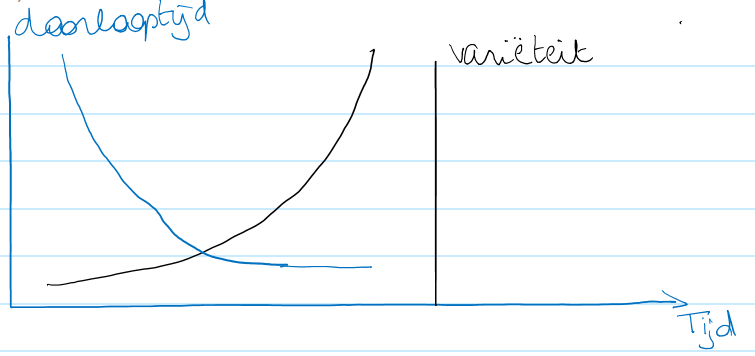
\includegraphics[width=90mm]{Les01_01.png}
\caption{Productlevencyclus} 
\label{les01_01}
\end{figure}

\paragraph{Slide 8:} Bedrijfseconomisch luik: voorspellingstechnieken: je hebt je product en je moet weten hoeveel je de komende maanden en jaren gaat produceren en welke consequenties daaraan hangen.\\
ERP: bv IER en ISP, personeelsbestanden, boekhouding,… 

\paragraph{Slide 10:} Set kleine vraagjes: vooral over begrippen (JIT, MRP,…). Let goed op verwoording en denk goed na over het antwoord! Bv: investering waarbij je 100 000 euro uitgeeft en je krijgt de volgende 5 jaar 30 000 terug, willen we nagaan of het interessant is. Als de waarde van het geld hetzelfde blijft, is het interessant. Kom niet af dat je rekenfouten gemaakt hebt op het examen!

\paragraph{Slide 13 $\&$ 14:}
\begin{itemize}
\item 5000 v.C. daar heeft men een aantal zaken teruggevonden die tonen dat men al bezig was met een soort boekhouding: bijhouden voorraden, leningen, uitgaven,… Daar werden dus al zaken opgevolgd.
\item Egyptische piramides: tonnen stenen moesten aangebracht worden, maar er waren ook enorm veel mensen aan het werken die moesten eten, slapen, verzorgd worden,…
\item 3000v.C.: volledig ontwikkeld staatssysteem.
\item Code van Hammurabi: men sprak al over minimumlonen.
\item Hannibal: logistieke organisatie om met heel die troep over te steken en eten te voorzien.
\item Feodale systemen: hi\"erarchische systemen: keizer met leenheren,… tot aan de lijfeigenen. De keizer kan niet alles voorzien dus gaat die een organisatiestructuur opbouwen die voor hem het best past. Je krijgt dan een baas die een aantal taken delegeert (bv. belastingen heffen, waarvan een deel moet worden afgestaan aan de keizer $\&$ manschappen sturen in tijden van oorlog).
\item 1300: dubbele boekhouding en kostberekeningen.
\item 1436: scheepswerf in Venetië: flowshop (alle producten volgen dezelfde weg: je hebt een aantal stations en men start met een skelet en op het einde heeft men een afgewerkte boot). Dit is zo'n bekend voorbeeld omdat er daar toen 2000 werknemers werkten en die slaagden erin om 100 boten te maken in minder dan 2 maanden. Er was dus een volledige organisatie van de lijn, de toevoer, het eten,…
\item 1700 e.v.: industri\"ele Revolutie: men bouwde stoommachines etc.: massaproductie. Men is gestart met gespecialiseerde taken, bouwmachines en massaproductie. Uitwisselbare stukken: men kan stukken gebruiken in verschillende machines: minder voorraad van die stukken nodig want je kan ze op meerdere plaatsen gebruiken. Bv kopiemachines: worden al voor 3e of 4e keer gebruikt. Zo'n 80\% van een oude machine is nog bruikbaar en wordt dus hergebruikt.
\item 1886: eerste keer ingenieur als economist $\rightarrow$ industrial engineering.
\item Henri Fayol: je moet denken aan productie, veiligheid, sturen plannen, accountancy,… $\rightarrow$ extra zaken die aan bod komen.
	\end{itemize}
	
\paragraph{Slide 15:} Ondernemen: er zijn mensen, materialen,…\\
Schumpeter: gebruikte de term ``ondernemer'' voor het eerst in de vorm van innovator. \\
Bedrijven worden alsmaar complexer $\&$ de klant komt meer centraal te staan: hij wil meer en sneller. Er wordt ook meer gekeken naar duurzame zaken. 

\paragraph{Slide 16:} Massaproductie etc kan problemen geven (realisatie) $\rightarrow$ biedt kortetermijnwinst. Er is dus langetermijnvisie nodig. \\
Henry Ford: als een bedrijf alleen maar winst wil maken, zou het eigenlijk niet mogen bestaan. Er is ook maatschappelijke bijdrage,… nodig. Toen is men de zaken anders beginnen bekijken.\\
Club van Rome: we moeten op een andere manier tewerk gaan om ervoor te zorgen dat we nog een paar 100 jaar kunnen voortgaan.

\paragraph{Slide 17:} Men moet duurzaam werken en men moet proberen voldoen aan de noden van vandaag op zo'n manier dat we de toekomst niet compromiteren.

\paragraph{Slide 19 - 22:} Veel bedrijven willen meewerken aan duurzaamheid. Als je hun jaarverslagen neemt, zie je dat ze daar ook over duurzaamheid praten.

\paragraph{Slide 23:} Een bedrijf staat niet op zichzelf dus je moet kijken naar de positie van de onderneming. Verschillende standpunten: gebruikers (mensen die producten aankopen: hebben bepaalde verwachtingen), de maatschappij (werkgelegenheid gewenst, diensten die iets voor hen doen), verwachtingen van het individu, markten (concurrenten!).\\
Een bedrijf is een economisch maar ook een sociaal systeem: zie \textbf{Slide 24:} aandachtspunten van Lotus op het sociaal systeem.

\paragraph{Slide 25:} Een bedrijf moet een meerwaarde cre\"eren, afkomstig van inkomsten en en uitgaven. Het verschil tussen beide is de meerwaarde. Je gebruikt die meerwaarde om lonen te betalen, belastingen, vergoeding voor het kapitaal, leningen $\&$ autofinanciering (kan gebruikt worden voor investeringen,…).

\paragraph{Slide 26:} Het bedrijf staat tussen leveranciers en klanten. Alle pijltjes zijn dingen die belangrijk zijn, bv levenscyclus: waar bevindt mijn product zich in de markt, wat is zijn levenscyclus?\\ Macht: ben je een grote klant van de leverancier of de enige klant? Dan kun je een aantal zaken doordrukken. Als je maar een kleine leverancier bent, dan zal dat minder zijn.

\paragraph{Slide 30:} Je kan intrapreneurship hebben (binnen een bedrijf) of erbuiten (entrepreneurship). In beide gevallen zoekt men naar innovatie. Schumpeter dacht dat dat vooral kon gevonden worden binnen bedrijven omdat er daar meer geld beschikbaar was. Dat is niet het geval. Naarmate een bedrijf groter wordt, wordt de organisatiestructuur logger en idee\"en die van werknemers komen, komen vaak niet tot ``boven''. In kleine bedrijven komt dat dus meer boven. Mensen die goede idee\"en hebben over aangepaste producten kunnen dat in een box steken in sommige bedrijven en zo gaat men die idee\"en evalueren.

\paragraph{Slide 31:} Een idee moet goed zijn en je moet ervoor zorgen dat de klant dat wil. Normaal moet het zo zijn dat jouw product het probleem van een klant oplost. Het moet een product zijn met duidelijke specificaties en het moet een potenti\"ele markt hebben. Ook rekening houden met concurrentie (bv. wasmachinetablet: vroeger was dat alleen maar in poeder en toen kwam Finish met tabletten en die begonnen 3 maand op voorhand daar reclame voor te maken. 1 week nadat het op de markt was gekomen, kwam een copycat er ook mee op de markt om dus ook een graantje mee te pikken. Het grote voordeel was dat de reclame gemaakt werd door Finish). Je moet voldoende beginkapitaal hebben (zelf hebben, binnenbrengen door investeerders aan te spreken,…). Je moet de juiste mensen aantrekken.

\section{Slides: 2\_Bedrijfskunde\_wat is een bedrijf}

\paragraph{Slide 5:} Er kunnen verschillende standpunten ingenomen worden om te kijken naar bedrijven. 

\paragraph{Slide 6:} De 4 sectoren: 2 laatste samen (tertiaire en kwartaire). De primaire sector neemt zo'n 3\% van BNP in beslag, de secundaire 33\% en de tertiaire en kwartaire de rest. De maatschappij is volledig veranderd van agrarisch naar dienstverlening.

\paragraph{Slide 7:} Je kan het bedrijf in 2 delen splitsen: goederen en diensten. De manier van werken en plannen is hier dikwijls anders. Als je kijkt naar ziekenhuizen, zij leveren ook diensten, dat is nog een stap verder dan hier. Als je naar een bank gaat voor een lening, negoti\"eer je. Als je naar een ziekenhuis gaat voor een operatie, ben je een product want je ondergaat de operatie. 

\paragraph{Slide 11 $\&$ 12:} Aangezien je niet aansprakelijk bent, word je veel meer gecontroleerd op wat je doet. 

\paragraph{Slide 13 e.v.:} Voor welk soort bedrijven.

\chapter{Les 2}

\section{Slides: 2\_Bedrijfskunde\_wat is een bedrijf}

\paragraph{Slide 19:} Onder kleine onderneming valt ook leverancier van brandstoffen (flexibeler).

\paragraph{Slide 23:} Interne jaarrekening: voor eigen gebruik.

\paragraph{Slide 24:} Marktstructuur: als je met een nieuw product op de markt wil komen, moet je rekening houden met het type markt. Als je kijkt naar volkomen concurrentie (een 100-tal spelers op de markt en de prijs wordt bepaald door de markt), als je daar op de markt wil komen, gaat niemand daar een probleem van maken (je moet gewoon zorgen dat kostprijs $>$ productieprijs). Bij een monopolie is dat anders: 1 partij bepaalt de prijs (op zo'n manier dat hij voldoende winst kan maken). Als er dan iemand op de markt komt met een gelijkaardig product, gaat de monopolist zijn prijzen laten dalen op zo'n manier dat hij bijna zeker is dat de nieuwkomer het product niet aan die prijze kan produceren (de monopolist kan in grote volumes produceren, de binnenkomer zeer waarschijnlijk nog niet). Bij een oligopolie zijn er een beperkt aantal spelers die de markt be\"invloeden. Daar binnengeraken is ook moeilijk, maar minder moeilijk dan bij een monopolie. Monopolistische concurrentie: afzetten van andere producenten door middel van productdifferentiatie.\\
$\Rightarrow$ Kijken hoe je je bedrijf moet organiseren om op de markt te kunnen komen.

\paragraph{Slide 25 e.v.:} Hoofdstuk 7 van Technische bedrijfsvoering $\&$ organisatie.

\paragraph{Slide 27:} Normaal heb je ergens een bepaalde visie, missie, strategie. Je gaat die dingen zo organiseren om je doelen te bereiken. Als je focust op verschillende producten moet je structuur dat ook weergeven.\\
Er zijn een aantal taken in verband met productie, verkoop en marketing $\rightarrow$ verantwoordelijkheden toewijzen en kijken hoe die zaken met elkaar communiceren.

\paragraph{Slide 28:} Organisatiehandleiding: taak- $\&$ functieomschrijving: elk bedrijf moet dat dus hebben. Ook bij KULeuven (onderwijsraad). Voor elke groep/functie bestaat dat. Ieder krijgt een instructieset met taken voor zijn/haar functie. Bij audits worden al die zaken ook gecontroleerd.

\paragraph{Slide 29:} Organisatieschema: bovenaan: algemeen directeur en per karakteristiek/element van het bedrijf een aantal afdelingen die uitgebouwd zijn. De personen die in een bepaalde silo zitten, gaan niet direct met andere mensen uit andere silo's spreken, dat zal via via verlopen.

\paragraph{Slide 31:} Lijnorg = volledig hi\"erarchisch. Een persoon onder een bepaalde persoon moet alleen luisteren naar die persoon en niet naar andere hogere functies waar hij/zij niet onder staat. $\rightarrow$ Duidelijke verantwoordelijkheidsbegrenzing: je gaat niet buiten je eigen gebied.

\paragraph{Slide 32:} Co\"ordinatie: als een uitvoerder naar een ``andere" baas moet gaan, zal dat via zijn baas moeten, dan naar directeur en zo naar die andere baas: grote omweg.
Zo'n structuur zal regelmatig wijzigen, is een levend organisme.\\
Omspanningsvermogen: hoeveel mensen kan ik overzien? Als je als afdelingshoofd makkelijk 15 mensen kunt opvolgen, maar als uw afdeling tot 25 mensen omvat, moet je die mss beter opsplitsen.\\
Spanwijdte: hoeveel mensen heb ik te overzien? Als spanwijdte $>$ omspanningsvermogen: beter op te splitsen.

\paragraph{Slide 33 $\&$ 34:} Speciale functie: staffunctie: ondersteunende functie (neemt zelf geen beslissingen, alleen raad en advies en schrijft documenten zodat een van de managers/directeurs dat kan gebruiken om bepaalde dingen door te drukken/voeren). Die verzamelt informatie, op systematische manier neerschrijven zodat de manager tot een besluit kan komen. Voordeel: het is nog steeds de manager/baas die beslist, de stafmederwerker neemt zelf geen beslissingen.

\paragraph{Slide 35:} Nadelen: draagt geen verantwoordelijkheden (de directeur is nog steeds de verantwoordelijke), het kan zijn dat je een fout overwicht krijgt: dat hij teveel overwicht krijgt op de manager.\\
Stafrelaties zijn voor advies, functionele relaties: diensten die dezelfde functiedeskundigheid hebben (bv. administratie). Men probeert binnen een bedrijf allemaal dezelfde documenten te gebruiken zodat die standaard zijn en makkelijk door te geven zijn zodat alles voor iedereen duidelijk is. Vroeger kon iedereen de dingen uitschrijven zoals men wou, tegenwoordig gaat dat niet meer, er zijn standaarden en het is voor iedereen hetzelfde.

\paragraph{Slide 37:} Een afdeling/bedrijf verandert qua structuur (bv. meer werknemers) en het overzien wordt misschien moeilijker. Decentralisatie is nodig wanneer dat beter past voor het type bedrijf om bepaalde zaken beter te kunnen uitvoeren. Soms is het beter eerst te decentraliseren en dan lokaal weer te centraliseren. $\rightarrow$ Je gaat alles mixen met elkaar.

\paragraph{Slide 41:} Functionele structuur: met departementen werken.

\paragraph{Slide 48:} Voordeel: groep mensen die gekoppeld zijn aan een project zelf. Nadeel: dubbele functies.

\paragraph{Slide 50:} Men laat de functionele structuur bestaan (mensen zitten in afdelingen), maar men gaat gebruik maken van die mensen op een horizontale manier. Voor projecten pikt men er dan mensen uit. Die mensen hebben nog altijd hun normale taken met daarbovenop extra taken voor het project (\textbf{Slide 53}). Matrixstructuur: verticale en horizontale taken.

\paragraph{Slide 54:} Men probeert meer en meer samen te werken (vroeger: leverancier was evil, wou gewoon winst maken). Men maakt speciale afspraken (bv. met VMI: Vendor Managed Inventory $\rightarrow$ de leverancier en het bedrijf werken samen. De leverancier weet hoeveel stukken er in het magazijn liggen en die kent het productieplan van het bedrijf (de klant) en kan zo zelf beslissen wanneer hij het magazijn gaat aanvullen wanneer dat het beste past in zijn planning. Moet er wel altijd voor zorgen dat er genoeg stukken liggen in het magazijn. De klant betaalt alleen voor wat hij gebruikt. Op die manier kan de leverancier zich beter organiseren. Bedrijven gaan elkaar soms ook overnemen om bepaalde zaken uit te voeren.\\
Horizontaal: leveranciers gaan samenwerken (bv. luchtvaartmaatschappijen: wisselstukken worden samen bekeken).

\paragraph{Slide 57:} Als je kijkt naar bedrijven, daar zijn een aantal functies (operations, marketing en finance). Die 3 moeten altijd op mekaar afgestemd zijn, anders raak je in de problemen. Bv. Apple: op een bepaald moment maakten ze reclame over het feit dat iedereen met een Apple kon werken. Dit sprak veel mensen aan en iedereen begon dat te bestellen. De computers werden geleverd (steeds met meer vertraging). Men dacht dat er een stijging ging zijn van de verkoop, maar marketing had het opgezet zonder te informeren bij de managers en financing. Men is veel gaan verkopen, maar men kon niet leveren. Er was dus geen cash flow. Men begon met de productie, maar omdat men dat te laat wist, kwam er een tekort waarbij men tot 6 maand moest wachten voor de pc geleverd kon worden.


\begin{figure}[h!]
\centering
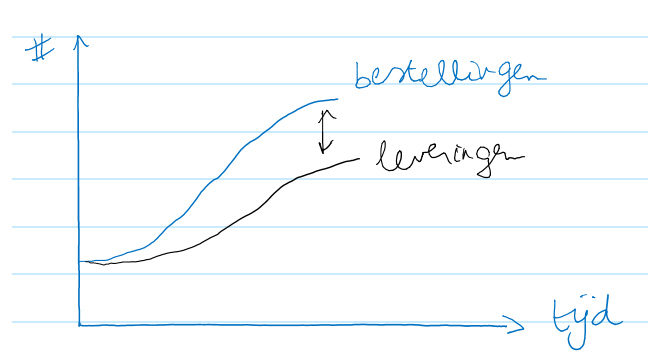
\includegraphics[width=90mm]{Les02_01.png}
\caption{Productlevencyclus} 
\label{les02_01}
\end{figure}


Dit was slechte reclame voor Apple: het was dan wel makkelijk om mee te werken, maar men moest er een half jaar op wachten.

\paragraph{Slide 58:} Bij massaproductie gaat men een lijn ontwikkelen om een bepaald product te ontwikkelen (bv. Ford Genk). Intermittent productie: het een is eenmalig, het ander is een grote batch. We hebben producten A, B, C waarbij een aantal stuks gemaakt moet worden. De productie moet zo gebeuren dat de voorraad beperkt is en de omstellingen die gemaakt moeten worden ook beperkt zijn. Je kan grote batches maken om minder omstellingen te hebben, maar dan heb je grote voorraden. Als je kleine voorraden maakt (dus kleine batches), heb je meer omstellingen en heb je te weinig tijd. De twee zijn dus tegenovergesteld aan elkaar. Je moet dit gaan optimaliseren.

\paragraph{Slide 59:} Strategische planning gaat kijken naar de impact op lange termijn (neemt niet per s\'e veel tijd in beslag!). Je moet kijken naar de tijdshorizon en zo objectieven vastleggen. Er is een hoge graad van onzekerheid omdat je over langere periodes gaat kijken, je weet niet altijd wat er juist gaat gebeuren. Het kan zijn dat men vrij goed kan voorspellen wat het verbruik gaat zijn bij klanten, maar niet per s\'e.\\
Tactische planning: wat als de verkoop cyclisch is: hoe ga je produceren? Ook cyclisch, of aan constante hoeveelheden?


\begin{figure}[h!]
\centering
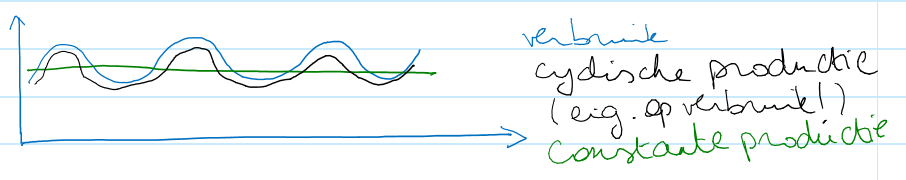
\includegraphics[width=90mm]{Les02_02.png}
\caption{Productlevencyclus} 
\label{les02_02}
\end{figure}


Normaal wordt eerst de strategische planning vastgelegd, dan tactische en dan operationele, maar het is niet puur sequentieel, het kan zijn dat men soms terugkoppelt en zaken aanpast.

\section{Slides: 3\_Bedrijfskunde\_Productlevenscyclus}

\paragraph{Slide 3:} Meestal komen producten er op basis van market pull, maar soms ook door de technologie zelf. Klanten vragen vaak zelf wel (market pull). Bij technology push gaat men proberen om noden te cre\"eren bij de klanten.

\paragraph{Slide 4:} De verschillende fasen: 
\begin{enumerate}
\item Introductie: product op de markt brengen. Hierbij is het dikwijls zo dat niemand het heeft en je moet dus zelf een prijs gaan bepalen. Als je zeker bent dat niemand het meteen gaat kopen, dan kan je de prijs relatief hoog zetten en meteen winst maken. Als het vervangbaar is door andere producten, is dat moeilijker. Als je start met een product is uw machinepark niet altijd correct afgesteld. Het product wordt dus vaak verkocht met verlies. Daarna kan je wel winst beginnen maken natuurlijk. 
\item Vroege groei: je moet nog oppassen voor copycats! 
\item Late groei: je moet je proberen differenti\"eren van andere bedrijven. Uw groei zal minder stijl zijn omdat er bv. concurrentie op de markt komt. Je zal dus minder verandering hebben, maar je moet ook kijken naar productie en financi\"en. Distributie komt hier ook bij kijken omdat je moet leveren aan de klanten.
\item Maturiteit: iedereen heeft het product en wat gekocht wordt is vervanging. Dan probeer je nog differentiatie te maken.
\item Eindstuk: iedereen is het product beu want er is een beter product op de markt, dus je kan verlies gaan lijden. Soms kan je hier geluk hebben: door je kostenstructuur te wijzigen kan je nog op een goede manier verkopen, ook als de verkoop daalt. Het kan dus zijn dat de interesse daalt, maar de marktpositie groeit nog wel.
\end{enumerate}

\paragraph{Slide 6:} Normaal, als je kijkt naar bedrijven die eerst op de markt zijn, die krijgen het grootste marktaandeel. Op de slide heb je bv. de cyclus van een bepaald product (PLC(1)), die ligt hoger dan die van PLC(2). 

\paragraph{Slide 7:} Men kan ook proberen van de levenscyclus te verlengen door er andere karakteristieken aan te geven. Bv. plakband: nieuwe versie op de markt brengen zodat het makkelijk af te scheuren is of zoiets. Zo ook met sigaretten bv. (met filter, minder teer,…).

\paragraph{Slide 8:} Niet alle curves lopen altijd hetzelfde: foothill: men brengt een product op de markt en sommige mensen moeten het dan hebben omdat het net op de markt is. Dan plots stopt het want niet iedereen is zeker of het interessant is of niet. Men wacht dan af wat de reactie is van de mensen die het al gekocht hebben. Het kan dan zijn dat het terug naar boven gaat (want positieve reacties van mensen die al gekocht hebben), of dat het niet goed is en dan daalt de curve (snel).

\paragraph{Slide 9:} Modeproducten: bv. geboorte prinses in Engeland: alle merchandise daarrond wordt enorm veel gekocht, iets later ineens niet meer. Hetzelfde verhaal met de hoolahoop.

\paragraph{Slide 10:} Grondstoffen en energiebronnen: hun gebruik is constant (olie, rubber, steenkool,…), ze zitten al lang in de maturiteitsfase.

\paragraph{Slide 11:} Als in de maturiteitsfase: flowshop maken dat specifiek gericht is op dat product. 
Je moet er rekening mee houden dat de PLC steeds korter worden, soms zijn producten al verouderd tegen dat ze op de markt komen.

\chapter{Les 3}

\section{Slides: 4\_algemene boekhouding} 

\paragraph{Slide 1} Bij een bedrijf moet je altijd een 5-jarig plan opstellen.

\paragraph{Slide 3:} We hebben een balans nodig omdat we willen weten wat er gebeurd is in het voorbije jaar. Een balans zit op strategisch niveau omdat we op lange termijn gaan kijken. Elk bedrijf moet zijn balans neerleggen bij de bank van Belgi\"e, maar vaak stelt men een tussentijdse balans op (bv. om de 3 maanden), zo kan men sneller ingrijpen indien nodig. \\
De bedoeling van algemene boekhouding is dat je ziet wat er juist gebeurd is binnen het bedrijf. Het is altijd van belang dat er een evenwicht is ($\sim$balans): we halen geld binnen (bronnen) en dat geld gebruiken we binnen ons bedrijf. De som van wat er binnenkomt moet gelijk zijn aan de som van wat we gebruiken.\\
Er zijn verschillende activiteiten die doorgaan tijdens een jaar (gewerkt, machinekosten,…) en we willen nagaan of die winstgevend zijn $\rightarrow$ resultatenrekening om te kijken of er winst gemaakt is of niet. Dan beslissen wat je met die winst gaat doen (uitkeren aan de aandeelhouders, uitgeven aan nieuwe investeringen,…).

\paragraph{Slide 4:} Figuur die het ondernemingsgebeuren weergeeft. Normaal is het zo dat als we willen produceren, we middelen moeten gebruiken om die productie te doen. Aan de ene kant interne middelen (mensen, machines) en aan de andere kant externe middelen (grondstoffen, gebruiksgoederen die zijn aangekocht). Deze middelen bepalen de kostprijs van ons product. Een deel van de middelen komt er via het verkopen van het product. Je moet weten wat de kostprijs is, welke winst je wil hebben en welke verkoopprijs je wilt. Deze laatste moet zo zijn dat je rekening houdt met uw positie in de markt.\\ Uiteindelijk komt het geld terug binnen (middelen voorgebracht door de activiteit).
Die geldstroom is enorm belangrijk: nodig om te investeren.

\paragraph{Slide 5:} We hebben een balans en resultatenrekening en we willen een samenvatting geven van wat er gebeurd is tijdens het jaar. We willen weten wat er gebeurd ismet de bezittingen en de vorderingen en het kapitaal.
Om de zaak aan te sturen zijn er de twee belangrijke principes.

\paragraph{Slide 6:} Je kan vanuit verschillende standpunten kijken naar een bedrijf (vanuit eigenaarsperspectief, banken,…).

\paragraph{Slide 7:} We hebben altijd een schuld tegenover eigenaars: zie Figuur \ref{les03_01}.

\begin{figure}[h!]
\centering
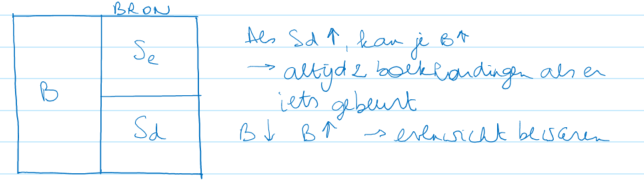
\includegraphics[width=90mm]{Les03_01.png}
\caption{Les 3 Slide 7} 
\label{les03_01}
\end{figure}

\paragraph{Slide 8:} De balans geeft altijd de zaken weer op een bepaald tijdstip (``foto"). Tussen 2 balansen (zoals hierboven getekend) heb je de resultatenrekening (geeft weer wat de activiteiten waren) en het journaal (houdt alles bij wat er gebeurt tussen 2 balansen). De balans is dus een momentopname, de resultatenrekening geeft meer de overgang aan.

\paragraph{Slide 9:} Balans: in een bepaalde volgorde (zie volgende slide). De passivazijde: staat gerangschikt volgens eisbaarheidsgraad. Het eigen vermogen is wat de personen die het bedrijf hebben opgericht hebben binnengebracht. Dat blijft in het bedrijf tot het bedrijf er eventueel mee stopt. Hoe verder naar beneden in de lijst, hoe sneller je die instantie moet terugbetalen.

\paragraph{Slide 11:} Als je kijkt naar een balans, moet dat op verschillende manieren: per kolom (anders bij dienstenbedrijven dan bij productiebedrijven). Het hangt er deels vanaf wat je gaat doen met uw winst. Je kan die bij de reserves gaan plaatsen (dan moet je die niet gaan uitbetalen), of aan dividenden (dan moet je dat uitbetalen aan de aandeelhouders). Als je de winst uitbetaalt, moet je 2000 terugbetalen op korte termijn. In principe zijn er genoeg middelen om de 2000 op korte termijn terug te betalen.
Je moet ook kijken over de tijdshorizon: naar de balans van dit jaar en van vorig jaar,… zo kan je evoluties binnen het bedrijf zien.

\paragraph{Slide 12:} Balansen van hetzelfde bedrijf, bekeken op verschillende tijdstippen. Het bedrijf werkt met seizoensgebonden vraag waarschijnlijk. Als je een piek hebt, moet je uw productieactiviteit daar niet naar aanpassen, je moet gewoon voorraad opbouwen in de magerdere periode (bv speelgoed): zie Figuur \ref{les03_02}.

\begin{figure}[h!]
\centering
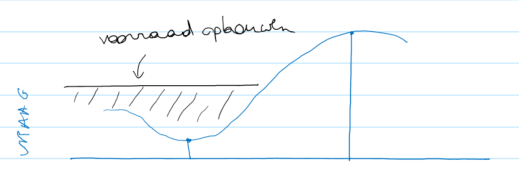
\includegraphics[width=90mm]{Les03_02.png}
\caption{Les 3 Slide 12} 
\label{les03_02}
\end{figure}

Je kan dus een totaal verschillend beeld krijgen wanneer je naar verschillende momenten in het jaar kijkt. 

\paragraph{Slide 13:} Je moet zorgen dat de balans eenduidig/juist is $\rightarrow$ wettelijke voorschriften.
\begin{itemize}
\item Informatiebron voor de bedrijfsleiding: keuzes etc.
\item Informatiebron voor diverse categorie\"en ge\"interesseerden: bv voor investeerders.
\end{itemize}
Als je een bedrijf opricht, moet je een ondernemingsplan oprichten en aantonen aan de bank dat je voldoende middelen hebt om de komende 5 jaar door te komen en dat je de interesten en aflossingen kunt afbetalen.
De overheid krijgt belastingen en als het goed gaat met het bedrijf zijn er werknemers die geen steun nodig hebben (en zij betalen ook belastingen).

\paragraph{Slide 14:} Er staan veel posten op de balans en die moeten op de juiste manier geschat worden.
\begin{itemize} 
\item Bedrijven kunnen hier laks in zijn, zeker als het gaat over financi\"ele activa (fluctueren dagelijks op de beurzen). 
\item Balanseenheid: moet eenduidig zijn en altijd hetzelfde stramien volgen. Als je lineair afschrijft (elk jaar hetzelfde bedrag), dan moet je dat elk jaar hetzelfde doen. Hetzelfde met de waardering van de voorraden. Eenmaal je gestart bent met een bepaalde regel, moet je die aanhouden $\rightarrow$ consistentie tussen verschillende balansen! Als je de regel wil aanpassen, moet je een aangepaste balans van vorig jaar geven zodat het opnieuw vergeleken kan worden.
\item Balansklaarheid: het moet duidelijk zijn wat er onder elke post staat. Als je een balans bekijkt heb je 2-3 pagina's overzicht en een 30-tal pagina's met verduidelijkingen van wat er juist bedoeld wordt.
\end{itemize}

\paragraph{Slide 15:} De sociale context is meer en meer aan het groeien.

\paragraph{Slide 17:} Zie Figuur \ref{les03_03}.

\begin{figure}[h!]
\centering
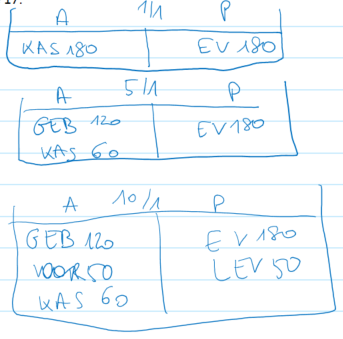
\includegraphics[width=90mm]{Les03_03.png}
\caption{Les 3 Slide 17} 
\label{les03_03}
\end{figure}

\paragraph{Slide 18:} Links altijd Debit, rechts altijd Credit (geheugensteuntje: denk aan prof zijn initialen).

\paragraph{Slide 19:} Creditzijde stijgt als we de bron laten stijgen.

\paragraph{Slide 20:} Resultatenrekening: kostenrekening en opbrengstenrekeningen: alles opgeteld. Opbrengst: credit + wat je moet aan de schuldeisers terugbetalen (je krijgt iets).

\paragraph{Slide 21:} Journaalboek waarbij alle transacties worden neergeschreven.

\paragraph{Slide 22:} Balans: alle boeken samenbrengen en alle saldi nemen en plaatsen in de balans en de resultatenrekening.

\paragraph{Slide 24 $\&$ 25:}
\begin{enumerate}
\item 2 posten: kas (dus kasboek nodig) en kapitaal.
\item Er wordt niet gespecifi\"eerd waar het geld terecht komt, dus we zetten het in de kas.
\item Er worden obligaties gekocht met geld uit de kas.
\item We hebben kosten gemaakt om producten aan te kopen, maar we hebben een voorraad en deltavoorraad liggen en 4 transacties. Alles in verband met voorraad en deltavoorraad wordt meestal apart gehouden. Wordt achteraf bekeken, rekening houdend met de waardering op dat momemt.
\end{enumerate}

Zie Figuur \ref{les03_04}, \ref{les03_05} $\&$ \ref{les03_06}.

\begin{figure}[h!]
\centering
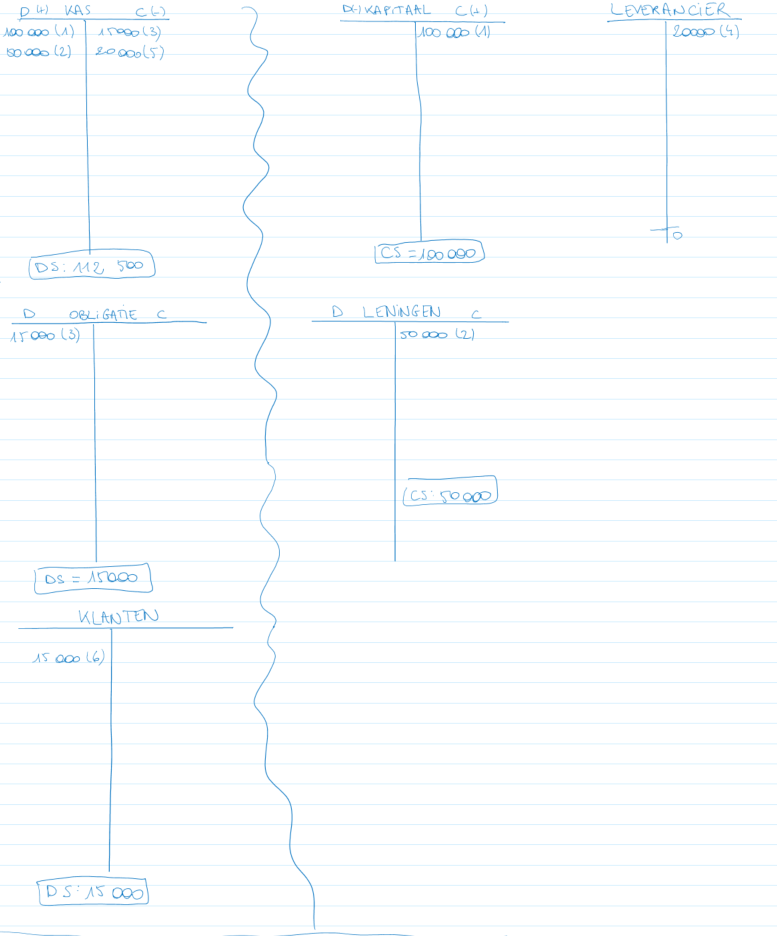
\includegraphics[width=90mm]{Les03_04.png}
\caption{Les 3 Slide 24 $\&$ 25} 
\label{les03_04}
\end{figure}

\begin{figure}[h!]
\centering
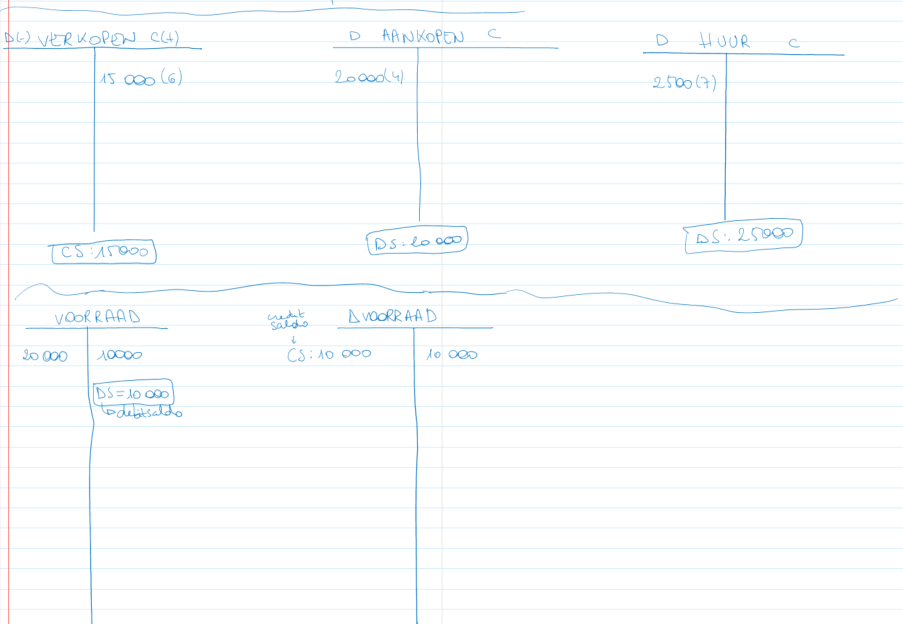
\includegraphics[width=90mm]{Les03_05.png}
\caption{Les 3 Slide 24 $\&$ 25} 
\label{les03_05}
\end{figure}

\begin{figure}[h!]
\centering
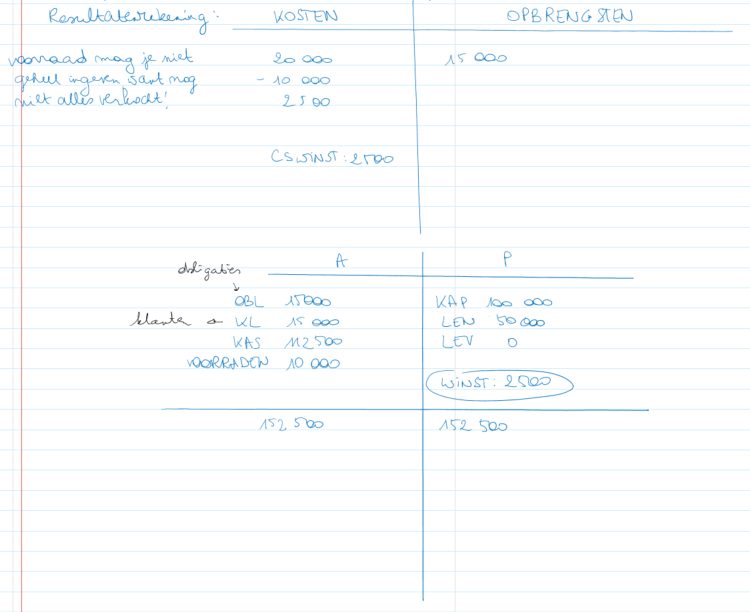
\includegraphics[width=90mm]{Les03_06.png}
\caption{Les 3 Slide 24 $\&$ 25} 
\label{les03_06}
\end{figure}

\paragraph{Slide 31:} Opgelet met voorraden: soms kan je de indruk krijgen dat je veel winst maakt terwijl dat niet zo is.

\paragraph{Slide 34:} Eerst wordt de resultatenrekening doorgerekend en dan wordt de nettowinst bekomen en die kan je opdelen in gereserveerde en verdeelde winst.

\section{Slides: 5\_Bedrijfskunde\_Financiele analyse en financiering}

\paragraph{Slide 2:} Men wil een balans tussen de eisbaarheid en de (???)graad..\\
De ratio-analyse is niet voor alle bedrijven hetzelfde, goed kijken naar de sector!\\
Financiering: we willen ervoor zorgen dat we voldoende cashflow hebben.

\paragraph{Slide 3: }
\begin{itemize}
\item Beleggers: ge\"interesseerd in beleggingen en kapitaalwinsten.
\item Schuldeisers willen hun geld terug, zijn ge\"interesseerd in rentabiliteit en de schuldenstructuur (als veel schulden: gaan niet direct willen investeren).
\end{itemize}

\chapter{Les 4}

\section{Slides: 5\_Bedrijfskunde\_Financiele analyse en financiering}

\paragraph{Slide 4:} Wij gaan naar de laatste 2 kijken.

\paragraph{Slide 5:} De actiefzijde en passiefzijde wijzigen op een jaar en je wil weten hoe dat gebeurd is, welke stromen voor die veranderingen hebben gezorgd.

\paragraph{Slide 6:} Figuur die ons vertelt hoe de kasstromen in elkaar zitten. Beneden is er de kas en daar kunnen er dingen de kas binnenkomen en verlaten.

\paragraph{Slide 7:} Als we kijken naar de balansen kunnen we ook kijken naar de mutatiebalans. We krijgen enkel de balans en geen omschrijving van wat er tijdens het jaar is gebeurd. We willen weten wat er is gebeurd met de activa en passiva. Kijken we naar materi\"ele vaste activa, zien we dat het bedrag met 250 gestegen is: er is een investering gebeurd (geld ergens vandaan gehaald en dat geld aangewend). Handelsvorderingen zijn ook gestegen: we verwachten nu nog meer geld terug van onze klanten (geld zit bij de klant). De voorraden zijn gedaald. Aanwending: stijging van de kosten, bron: daling.\\
Passiefkant: schulden op meer dan 1 jaar: die zijn gestegen: we hebben ergens meer geld binnengehaald en dat is een bron van inkomsten. De schulden $<$ 1 jaar zijn gedaald (die zijn terugbetaald). Als een bron stijgt, stijgen de passiva.\\
Ook van belang is een aanwending van 250 vaste activa.

\paragraph{Slide 8:} Let op: de totalen zijn gelijk aan die van in \textbf{Slide 7}!

\paragraph{Slide 9:} We gaan sterktes en zwaktes proberen afleiden op basis van ratio's (kerngetallen). Je kan die ratio's ook overheen de tijd bekijken en tussen verschillende ondernemingen maar wel best binnen dezelfde sector.

\paragraph{Slide 10:} We willen dat de kanten aan elkaar gelijk zijn (ook binnen de hokjes zelf, niet alleen in totaal), zo willen we bv. dat we onze schulden zo snel mogelijk kunnen terugbetalen. 

\paragraph{Slide 11:} Schulden op korte termijn terugbetaald en we hebben zo nog 80 overgehouden: er zijn reserves.

\paragraph{Slide 12:} In \textbf{Slide 10} hebben we een bedrijfskapitaal van 0 omdat we alles nodig hebben om de schulden terug te betalen. In \textbf{Slide 11} is het bedrijfskapitaal 80 omdat er dus nog over is.\\
Relatieve vorm: geeft de vergelijking aan. Als die groter is dan 1, is het bedrijfskapitaal dus positief.\\

\paragraph{Slide 13:} Je krijgt uw geld pas op het einde van de onderste lijn terug: je moet heel die periode dus overbruggen. Hoe langer die periode, hoe slechter voor je bedrijf. Je kan die inkorten door de productie sneller te laten worden, de voorraden kleiner te laten worden, leverancierskrediet groter te maken of het klantenkrediet kleiner te maken. Kan die periode negatief worden? Ja, bv. in winkels. Bedrijven als Colruyt hebben meestal contracten van 60 tot 90 dagen (dus na 90 dagen betalen ze de leveranciers). De voorraad ligt er meestal 2 weken (dus 14 dagen). De klant betaalt meteen (dus na 14 dagen). Dit wilt zeggen dat de winkels geld hebben ontvangen voor dingen die ze zelf nog niet hebben afbetaald. Zie Figuur \ref{les04_01}

\begin{figure}[h!]
\centering
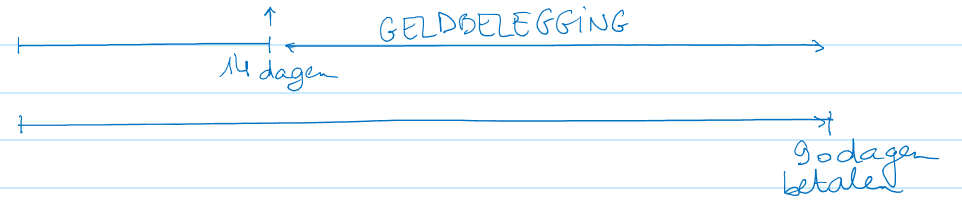
\includegraphics[width=90mm]{Les04_01.png}
\caption{Les 4 Slide 13} 
\label{les04_01}
\end{figure}

\paragraph{Slide 14:} Voorraadrotatie willen we liefst hoog, dan hebben we een kleine gemiddelde voorraad, dus deze roteert snel. We gaan de voorraad in het bedrijf inkorten (op de tekening hierboven zou het dus ook maar een aantal dagen zijn). Bv. zie Figuur \ref{les04_02}.

\begin{figure}[h!]
\centering
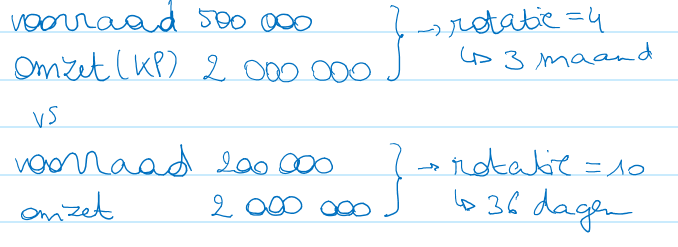
\includegraphics[width=90mm]{Les04_02.png}
\caption{Les 4 Slide 14} 
\label{les04_02}
\end{figure}

Klantenrotatie willen we zo klein mogelijk hebben (dan betalen ze sneller). 
Als je kijkt naar de tapijtindustrie en de voorraadperiode (VP),  het leverancierskrediet (LK) en het klantenkrediet (KK), dan liggen de tapijten er meestal 75 dagen, de leveranciers worden na 83 dagen betaald en de klanten betalen na 85 dagen. In tabelvorm:


\begin{table}[h!]
\centering
\begin{tabular}{|c||c|c|c|}
\hline                         										
		 				&	VP 		&	LK		&	KK		\\	\hline	\hline
Tapijt					&	75		&	83		&	85		\\	\hline
Kleinhandel Voeding		&	29		&	61		&	10		\\	\hline

\end{tabular}
\label{les4_slide14}
\end{table}

\paragraph{Slide 15:} Schuldenratio moet zo laag mogelijk zijn (niet teveel vertrouwen op externe financiering), solvabiliteitsratio moet zo hoog mogelijk zijn.\\
Toegevoegde waarde: deze wordt gebruikt om lonen te betalen, de staat te betalen,…

\paragraph{Slide 16:} De autofinanciering is interessant: kan gebruikt worden om verdere financieringen door te voeren.

\paragraph{Slide 17:} Afschrijvingen worden afgeschreven als kost maar ze zijn geen cash flow. Als je een investering doet van 1 miljoen, betaal je dat en gedurende de volgende jaren mag je bv. 100 000 afschrijven. Dit is een recuperatie van gemaakte investeringskosten, maar dat is dus geen nieuw geld dat binnenkomt.

\paragraph{Slide 21:} Grafisch voorstellen van wat daar ook staat: zie Figuur \ref{les04_03}.

\begin{figure}[h!]
\centering
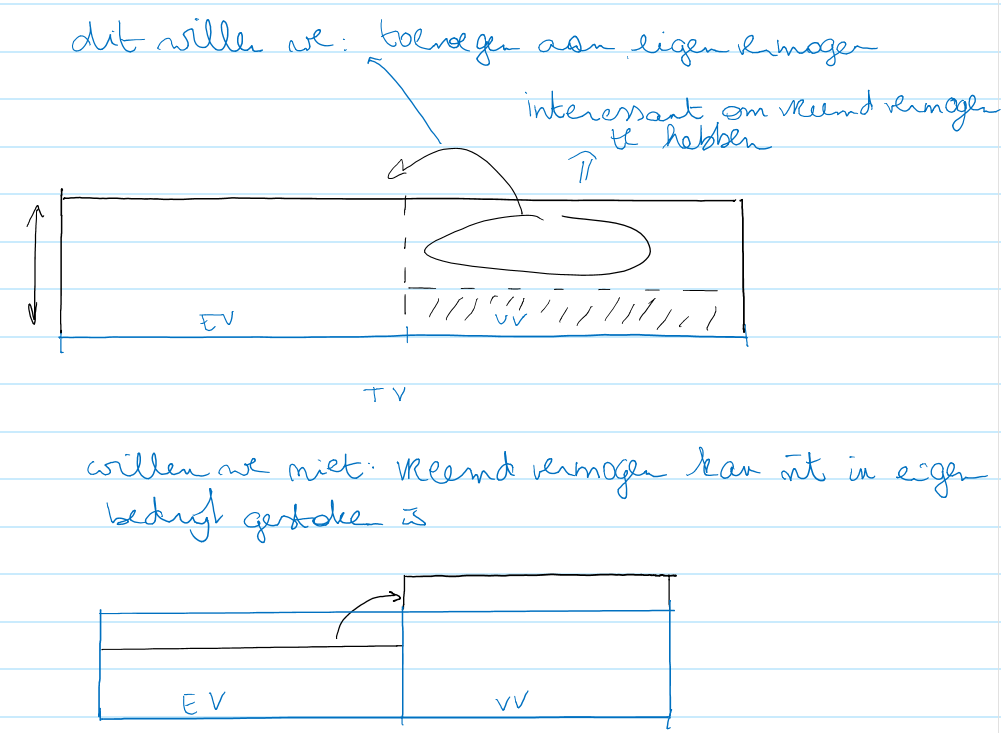
\includegraphics[width=90mm]{Les04_03.png}
\caption{Les 4 Slide 21} 
\label{les04_03}
\end{figure}

\paragraph{Slide 22:} Balans op 31/12 die jaren x en x+1 toont.

\paragraph{Slide 23:} Zie Figuur \ref{les04_04}, \ref{les04_05} $\&$ \ref{les04_06}.

\begin{figure}[h!]
\centering
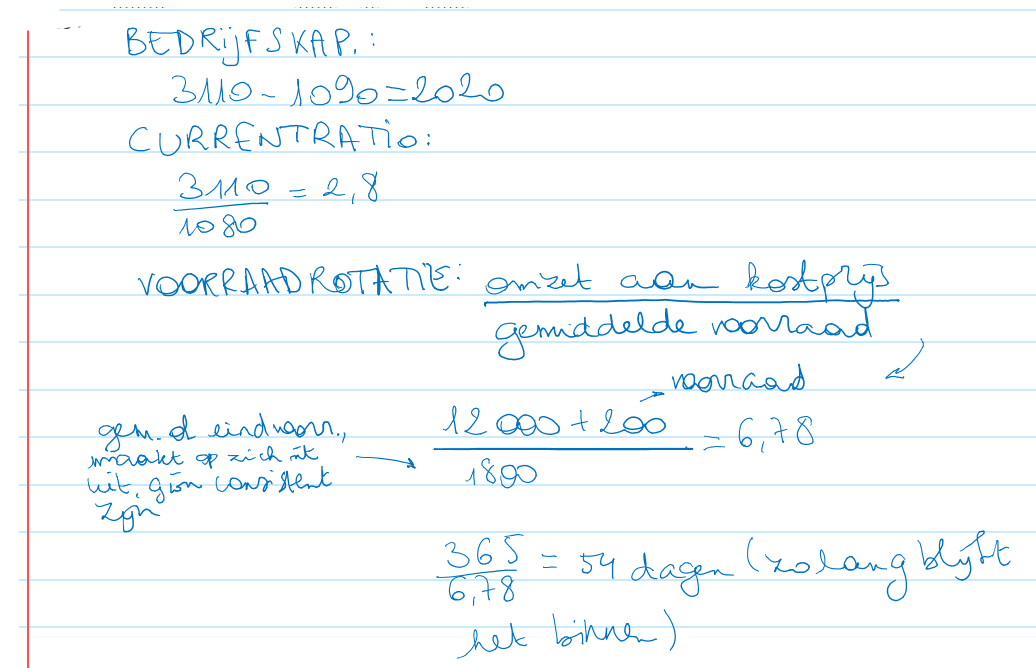
\includegraphics[width=90mm]{Les04_04.png}
\caption{Les 4 Slide 23} 
\label{les04_04}
\end{figure}

\begin{figure}[h!]
\centering
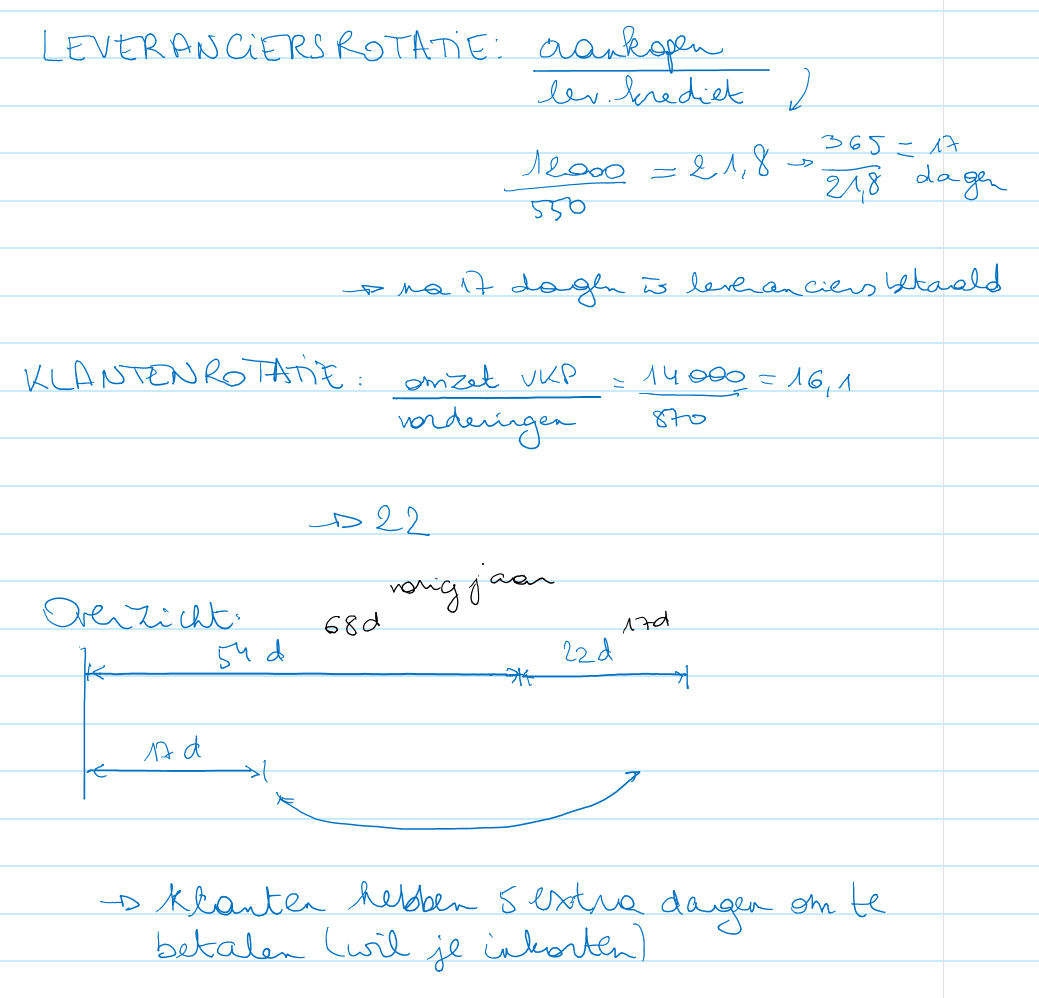
\includegraphics[width=90mm]{Les04_05.png}
\caption{Les 4 Slide 23} 
\label{les04_05}
\end{figure}

\begin{figure}[h!]
\centering
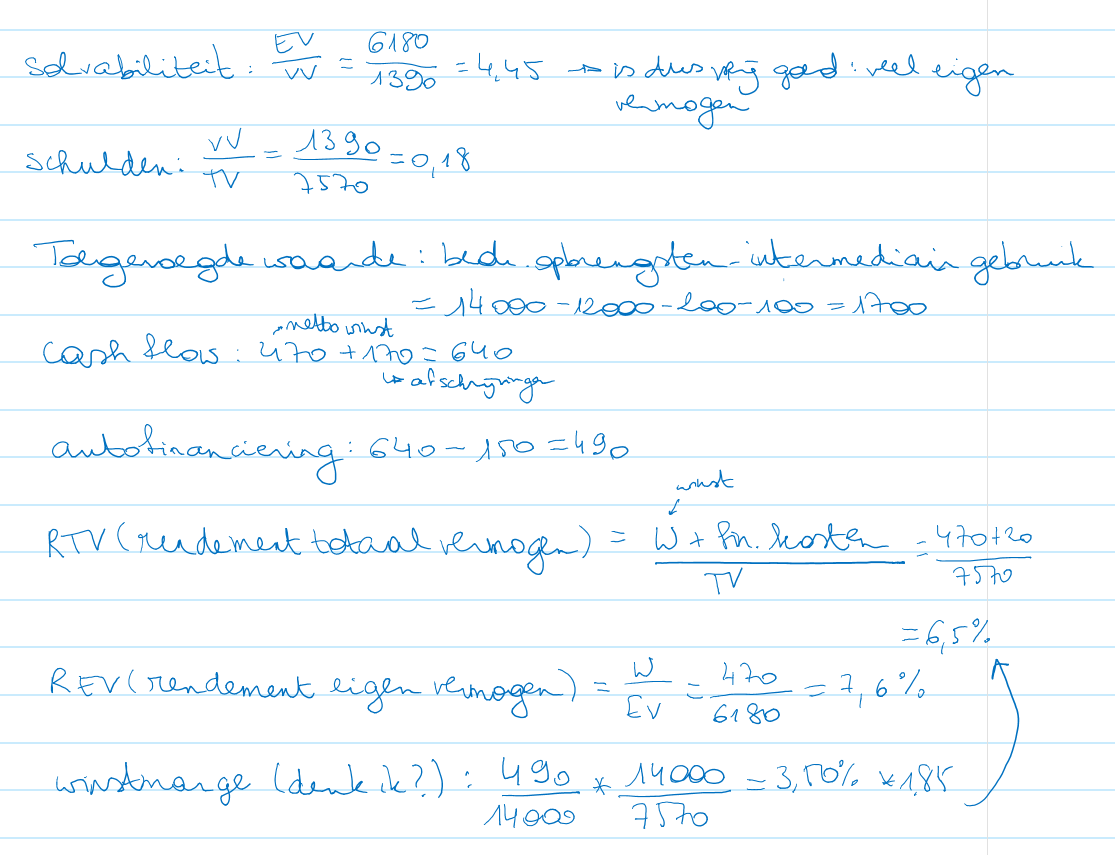
\includegraphics[width=90mm]{Les04_06.png}
\caption{Les 4 Slide 23} 
\label{les04_06}
\end{figure}

\paragraph{Slide 25:} Je moet elk jaar beslissen of je dividenden gaat uitbetalen of niet (staat dus niet vast). Obligaties moeten terugbetaald worden, aandelen niet.

\paragraph{Slide 26:} Rekening-courant: je hebt x euro staan en naarmate je daar gebruik van maakt, zoveel interest betaal je daarop.

\chapter{Les 5}

\section{Slides: 6\_Bedrijfskunde\_Kostprijssystemen}

\paragraph{Slide 3:} Structuurbeslissingen: investeringen doen, deze hebben invloed op de kostprijs. Het is de bedoeling dat we de kost kennen van elk product (maar dit is niet eenduidig!).\\
Kostenbeheer van elke afdeling: elke afdeling heeft vaste kosten en variabele kosten. We willen zien of deze zaken optimaal worden ingezet.

\paragraph{Slide 4:} Voor ons is het eerste puntje minder interessant. Wij zijn meer ge\"interesseerd in puntje 2 $\&$ 3. Toewijsbaarheid: als je denkt aan de grondstoffen en daar is een product van gemaakt, wil je weten hoeveel grondstoffen daar naartoe zijn gegaan.

\paragraph{Slide 5:} Je kan uw elementen opsplitsen. Het meest rechtse is een combinatie van het linkse en het middelste. Vaste indirecte kosten: bv. gebouwen (je kan niet meteen zeggen voor welk product dat gebouw dient). Let op: als we spreken over indirecte kosten, gaat het normaal over een bedrijf dat meer dan 1 product maakt. Als het bedrijf maar 1 product maakt, is alles direct toewijsbaar, heb je geen indirecte kosten.

\paragraph{Slide 6:} Bij vaste kosten maakt het niet uit hoeveel producten je maakt, de kosten blijven hetzelfde.

\paragraph{Slide 7:} Er kan een sprong inzitten, bv. omdat uw magazijn te klein is geworden, dus verhuis je naar een groter magazijn, maar dan wordt uw kost weer vast.

\paragraph{Slide 8:} Variabele kosten: die zullen meestal proportioneel zijn met de productie. Soms kan het zijn dat er een extra stijging is, als je dicht bij de maximale capaciteit zit (progressief). Het kan ook zijn dat je een afname hebt wanneer je bv. grondstoffen moet aankopen en bij het aankopen van grote batches krijg je korting (degressief). 

\paragraph{Slide 9:}
\begin{itemize}
\item Directe kosten: zijn rechtstreeks toewijsbaar. Voorraden moet je wel apart houden omdat je rekening moet houden met de voorraadwaardering.
\item Directe materiaalkosten: we werken hier met FIFO (we kijken naar de oudste producten eerst en we kijken ook naar de waarde van de grondstoffen op dat moment) en LIFO (omgekeerd).
\end{itemize}

\paragraph{Slide 10:} Je gaat bij t2 maar 1000 aankopen in plaats van meteen 2000.

\paragraph{Slide 11:} Identiek dezelfde aankopen en verkopen, maar de 4000 van t3 wordt eerst uit t2 en t1 genomen.\\
Afhankelijk van de situatie (moet vermeld staan op de balans) moet je rekening houden met wat je doet.\\
FIFO en LIFO is puur boekhoudkundig! Als we dus met LIFO werken en we hebben een bedrijf dat yoghurt verkoopt, wil dat niet zeggen dat ze alleen de meest verse zullen verkopen. Boekhoudkundig zal er misschien wel LIFO gebruikt worden, maar fysisch FIFO.

\paragraph{Slide 12:} Je kan verschillende manieren gebruiken, maar je moet altijd consistent zijn en het moet ergens neergeschreven staan.

\paragraph{Slide 13:} Als iemand aan een bepaalde productielijn staat, weet je waar dat geld naartoe gaat. \\
Indirecte kosten: moeilijker om toe te wijzen. Je moet uitvissen waarom je een kost zou toewijzen aan een bepaald proces of product. Vroeger kon men zeggen dat 90\% van de kosten direct toewijsbaar was (kleine fout). Als je nu gaat kijken naar bedrijven, is dat sterk veranderd: meer dan de helft van de kosten zijn nu indirecte kosten. Vandaar dat je ook grotere afwijkingen kunt krijgen op uw kosten.

\paragraph{Slide 14:}
\begin{itemize}
\item Primitieve toeslagmethode:
\begin{itemize}
\item We kunnen kijken naar de directe loonkosten als dat de belangrijkste parameter is binnen het bedrijf. 
\item Per eenheid eindproductie: we maken van alles samen 5000 stuks, deel indirecte kosten door 5000 en verdeel het.
\item Toeslag op basis van directe materiaalkosten: indirecte kosten zijn gerelateerd aan de directe materiaalkosten of (lonen?).
\item Op basis van directe kosten: som van beide.
\end{itemize}
\item Verfijnde toeslagmethoden: indirecte kosten meer en meer proberen uitsplitsen.
\end{itemize}

\paragraph{Slide 15:} Ondersteuningscentra: proberen toewijzen aan de hoofdcentra. Laatste: kan je niet meteen toewijzen. Zie kader rechts.

\paragraph{Slide 16:} Voorbeeld: smederij: cijfers achter rode lijn zijn niet meegeteld in het totaal (naast sleutel).
\% directe lonen: je gaat je indirecte lonen berekenen aan de hand van een percentage van de directe lonen (ongeveer 1/8 hier: alle indirecte lonen zullen ongeveer 1/8 van de directe lonen zijn).

\paragraph{Slide 17:} Zie Figuur \ref{les05_01}, \ref{les05_02} $\&$ \ref{les05_03}.

\begin{figure}[h!]
\centering
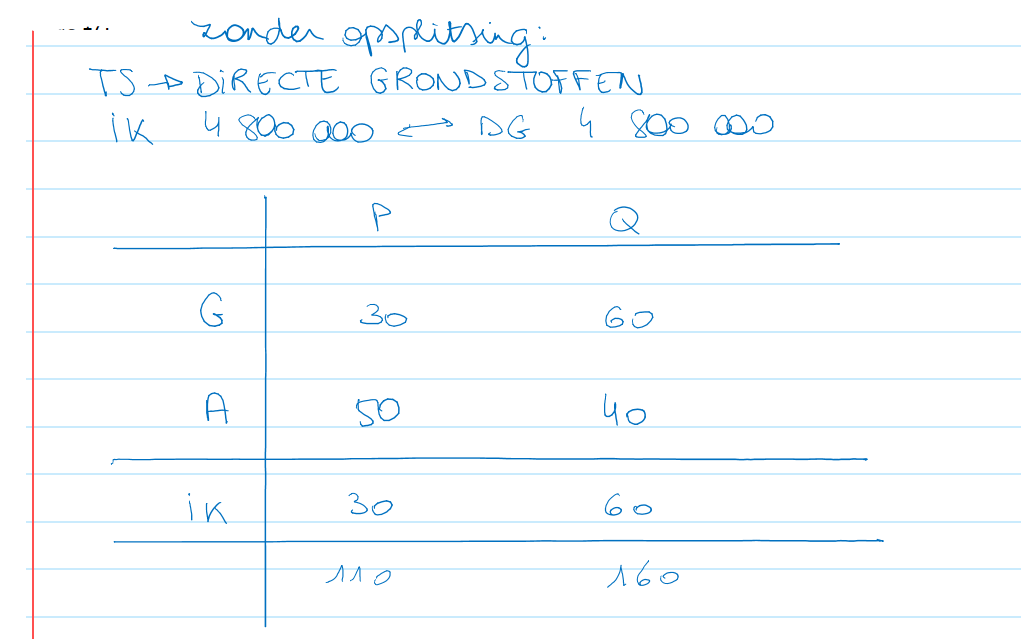
\includegraphics[width=90mm]{Les05_01.png}
\caption{Les 5 Slide 17} 
\label{les05_01}
\end{figure}

\begin{figure}[h!]
\centering
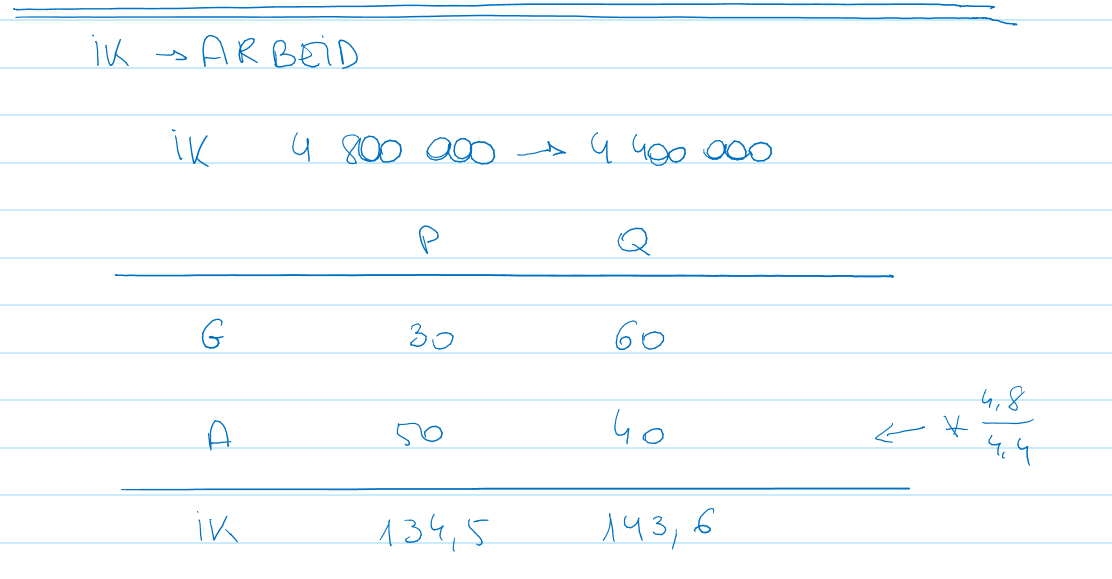
\includegraphics[width=90mm]{Les05_02.png}
\caption{Les 5 Slide 17} 
\label{les05_02}
\end{figure}

\begin{figure}[h!]
\centering
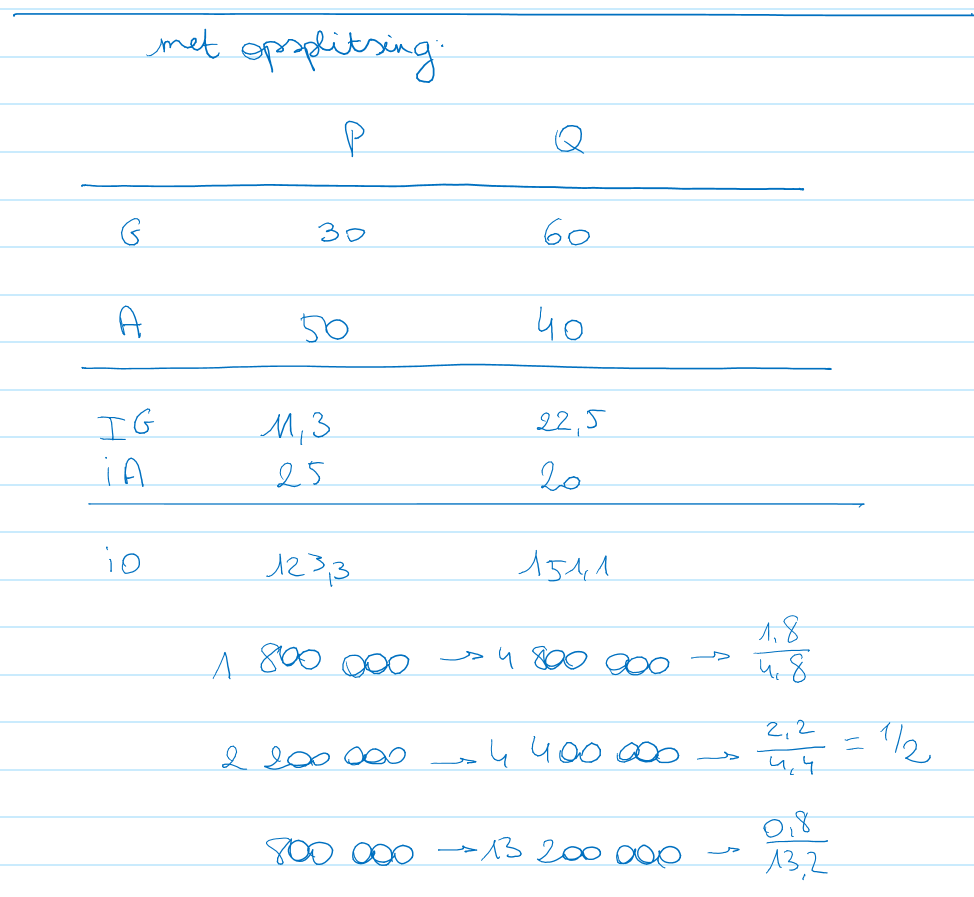
\includegraphics[width=90mm]{Les05_03.png}
\caption{Les 5 Slide 17} 
\label{les05_03}
\end{figure}

\paragraph{Slide 21:} 250 000: eerste getal vermenigvuldigd met 40 000 en het tweede getal vermenigvuldigd met 60 000.

\paragraph{Slide 22:} Zie Figuur \ref{les05_04}.

\begin{figure}[h!]
\centering
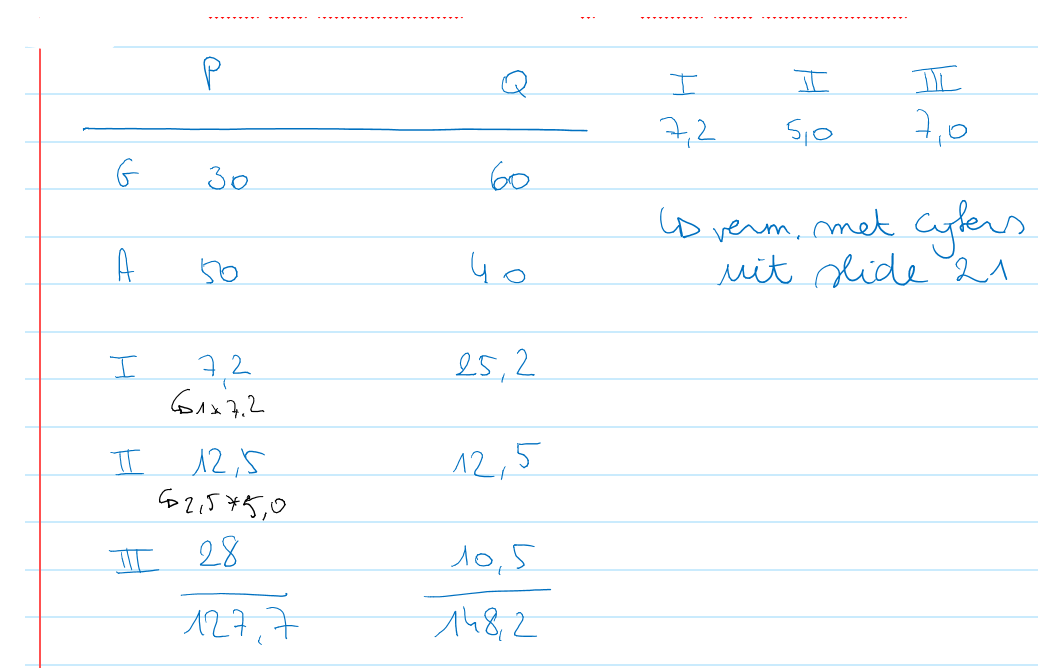
\includegraphics[width=90mm]{Les05_04.png}
\caption{Les 5 Slide 22} 
\label{les05_04}
\end{figure}

\paragraph{Slide 24:} Als je een bepaalde investering doet, wordt dat niet onmiddelijk ingebracht. Je brengt achteraf afschrijvingen in (gebouw, machine,…). De kasstroom gebeurt op het moment van investeren. Je hebt verschillende definities zoals getoond op de slide.

\paragraph{Slide 25:} Zie Figuur \ref{les05_05}.


\begin{figure}[h!]
\centering
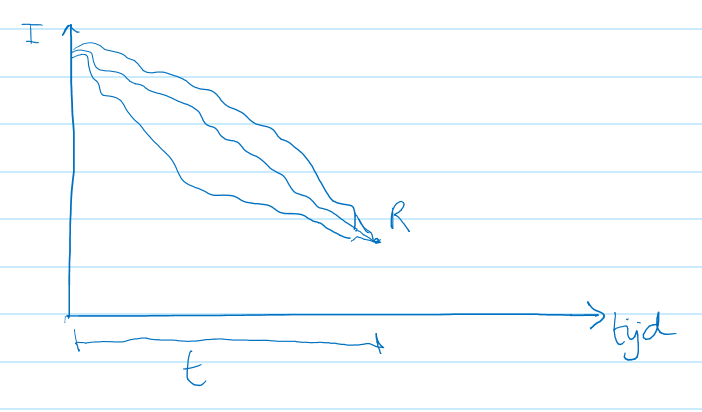
\includegraphics[width=90mm]{Les05_05.png}
\caption{Les 5 Slide 25} 
\label{les05_05}
\end{figure}

\paragraph{Slide 27:} Afschrijvingsperiode: kan vari\"eren: voor machines kan dat 5 jaar zijn, voor gebouwen 30 jaar. Hangt ook af van de fysische of technische levensduur: een wagen kan bv. afgeschreven worden na 5 jaar. %Economische levensduur: de machine (???)
%Fiscale levensduur

\paragraph{Slide 28:} Lineair afschrijven: bepaald investeringsbedrag, product gaat 10 jaar mee. Zie Figuur \ref{les05_06}.

\begin{figure}[h!]
\centering
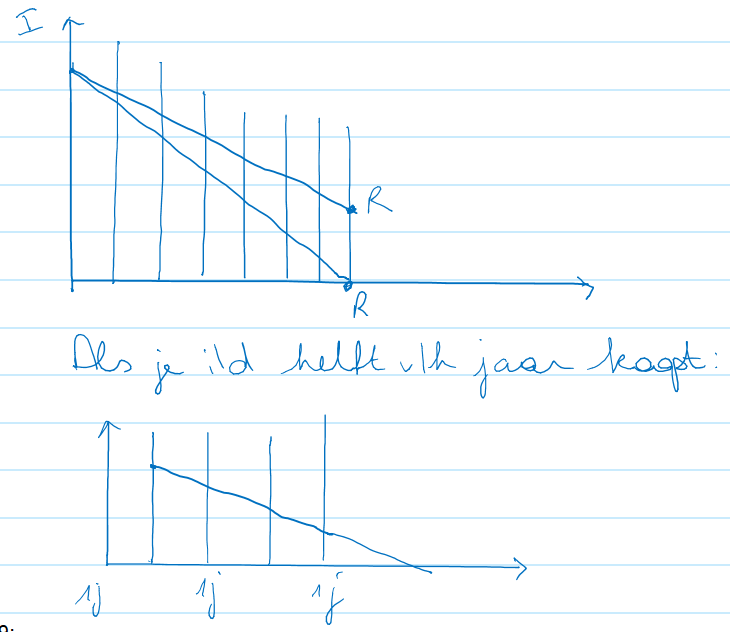
\includegraphics[width=90mm]{Les05_06.png}
\caption{Les 5 Slide 28} 
\label{les05_06}
\end{figure}

\paragraph{Slide 29:} Zie Figuur \ref{les05_07}.

\begin{figure}[h!]
\centering
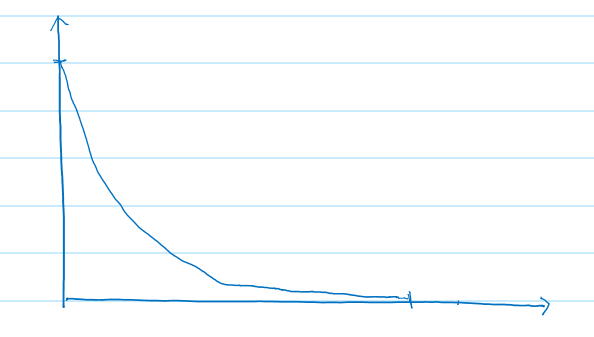
\includegraphics[width=90mm]{Les05_07.png}
\caption{Les 5 Slide 29} 
\label{les05_07}
\end{figure}

\paragraph{Slide 30:} Voorbeeld: elk jaar schrijven we 100 af. Ook mogelijk: zie Figuur \ref{les05_08}.

\begin{figure}[h!]
\centering
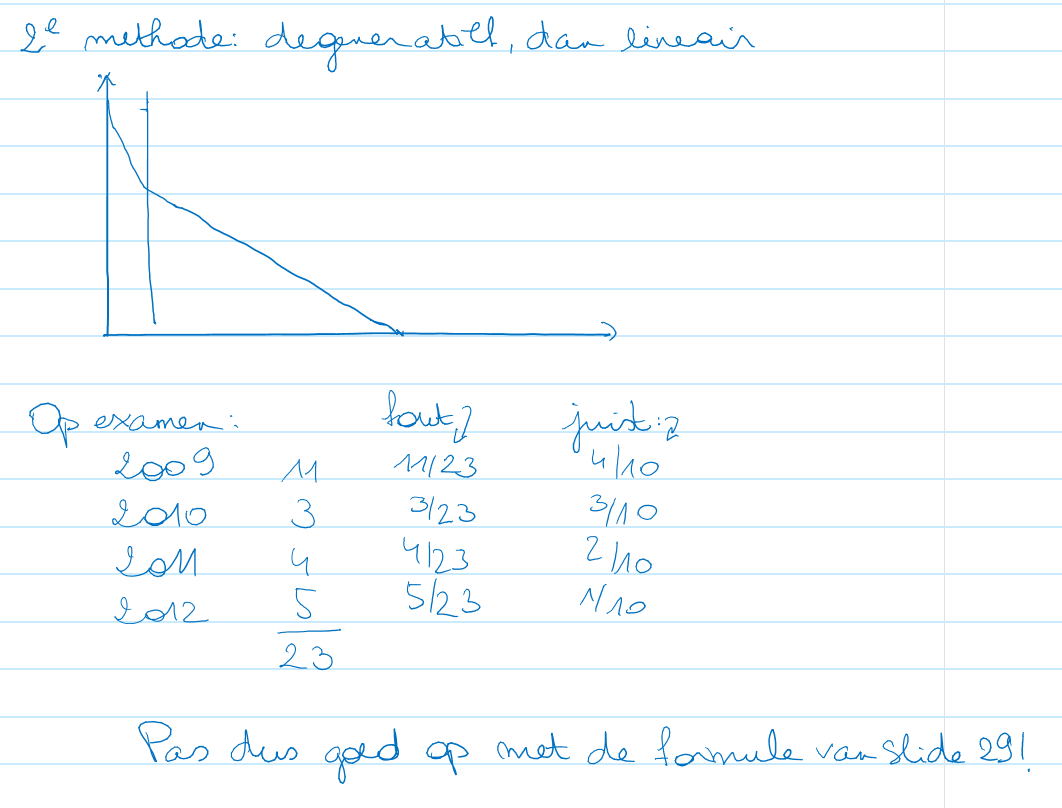
\includegraphics[width=90mm]{Les05_08.png}
\caption{Les 5 Slide 30} 
\label{les05_08}
\end{figure}

\paragraph{Slide 31:}
\begin{itemize}
\item Klassieke totale kostprijs: daar zit alles in (zeg dus niet dat er zaken niet inzitten).
\item Industri\"ele kostprijs: bevat alleen de productiekosten: alle kosten zonder algemene kosten en verkoop.
\item Evenredige kostprijs: enkel de kosten die evenredig zijn met de hoeveelheid van elk product. Deze is dus de kleinste, de industri\"ele kosten zijn al wat hoger en de klassieke kosten zijn de hoogste.
\end{itemize}

\paragraph{Slide 32:} De totale kostprijs kan je maar bepalen als alles gebeurd is. Normaal moet je alle postenkosten kennen. Daarom spreekt men over de historische totale kostprijs. Bij industri\"ele en evenredige standaardkostprijs gaat men kijken naar de toekomst.

\paragraph{Slide 34:} Er zijn altijd voor- en nadelen! Afhankelijk van de seizoensperiode kunnen de prijzen vari\"eren omdat men meer/minder stuks maakt. Historisch komt eigenlijk te laat.\\
Ook vervelend: doordat men alles gaat optellen weet je niet goed van waar het allemaal komt. Je hebt dus ook geen verantwoordelijke.

\paragraph{Slide 35:} Als je een full cost berekend hebt, hoe moet je die gaan vergelijken met de kostprijs? Als je variabele kosten van 50 hebt en vaste kosten van 50 en een full cost van 100, terwijl de verkoopprijs 90 is, dan is dat (g?)een slechte zaak. Je moet altijd zorgen dat de verkoopprijs groter is dan uw variabele kost. De vaste kosten zijn toegewezen aan een aantal producten dat je maakt. Als je meer producten gaat produceren, gaan die totale vaste kosten dalen.\\ Normaal hebben we een vaste kost en een variabele kost. Als we een aantal stuks produceren, dan is de totale kost aangeduid op de tekening (1) en de full kost is (2). Als we tot de conclusie komen dat we een verkoopprijs hebben die eronder ligt (3), dan maken we verlies. Als we meer stuks kunnen verkopen en produceren kunnen we wel nog aan winst komen. Zolang de verkoopprijs groter is dan de variabele kosten, wordt nog altijd een deel van de variabele kosten gedekt. Zie Figuur \ref{les05_09}.

\begin{figure}[h!]
\centering
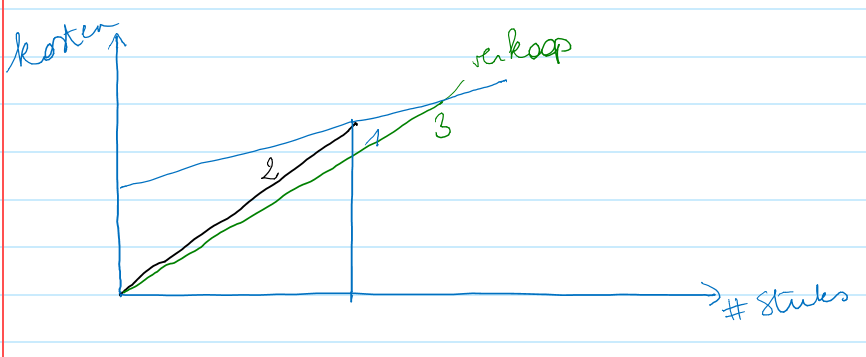
\includegraphics[width=90mm]{Les05_09.png}
\caption{Les 5 Slide 35} 
\label{les05_09}
\end{figure}

\paragraph{Slide 36:} B niet meer verkopen zal ervoor zorgen dat A ook niet meer rendabel is. Het ligt aan uw kostentoewijzing (denk ik).

\paragraph{Slide 39:} Industri\"ele standaardkostprijs: ontstaan op basis van kostenplaatsmethode en standaarden van technische gegevens. Je gaat een schatting maken, dus er zal een verschil zijn tussen de geschatte en de werkelijke kostprijs. Je gaat alles in detail analyseren. 

\paragraph{Slide 40:} Tabel van daarnet.

\paragraph{Slide 41:} Administratieve zaken en verkoop zitten niet in de industri\"ele standaardkostprijs (laatste kolom op \textbf{Slide 40}).

\paragraph{Slide 44:} Er wordt enkel naar de variabele kosten gekeken en die gaan we toewijzen aan kostendragers. Vaste kosten worden naar de resultatenrekening afgevoerd.

\paragraph{Slide 45:} Voordelen:
\begin{itemize}
\item Er wordt een expliciete relatie tussen volumes, kosten en winst gemaakt.
\item Je kan kijken of je korting gaat geven aan een bepaalde klant: je weet wat de marges zijn.
\item Kostencontrole wordt makkelijk.
\end{itemize}

\paragraph{Slide 46:} Prijzen niet altijd laten dalen want dan kan het zijn dat de vaste kosten niet meer gedekt worden. Je mag de vaste kosten dus niet uit het oog verliezen, die zijn er natuurlijk nog altijd.\\
Stel je hebt product A en B. A geeft 3 euro winst per stuk en B 7 euro. Je gaat dus B meer maken en proberen verkopen (intu\"itief). Je weet niet hoeveel uur je nodig hebt om beide te produceren (stel A heeft slechts 1 uur nodig en B 30 uur, dan is A interessanter). Pas dus op met de evenredige kostprijs!

\paragraph{Slide 47:} Je hebt uw vaste kosten (verticale as tot aan C(q) en de variabele kosten (C(q) ). Zodra je meer produceert dan q* maak je winst. 

\paragraph{Slide 48:} Je moet altijd zorgen dat je kostenstructuur goed zit. Hotels hebben bv. veel vaste kosten. Dit zorgt voor een andere gevoeligheid van het dode punt. Je kan ook verschillende snijpunten krijgen, zie \textbf{Slide 49}.

\paragraph{Slide 49:} Als de vaste kosten een sprong krijgen, kan het dode punt verschuiven. Het kan zijn dat de kostenstructuur van de variabele kosten niet altijd lineair verloopt, maar dicht ligt aan de capaciteitskosten en dat je bv. overuren moet doen en dan kan je dus meer kosten hebben.

\chapter{Les 6: Oefenzitting 1}
Zie volgende pagina voor handgeschreven nota's.

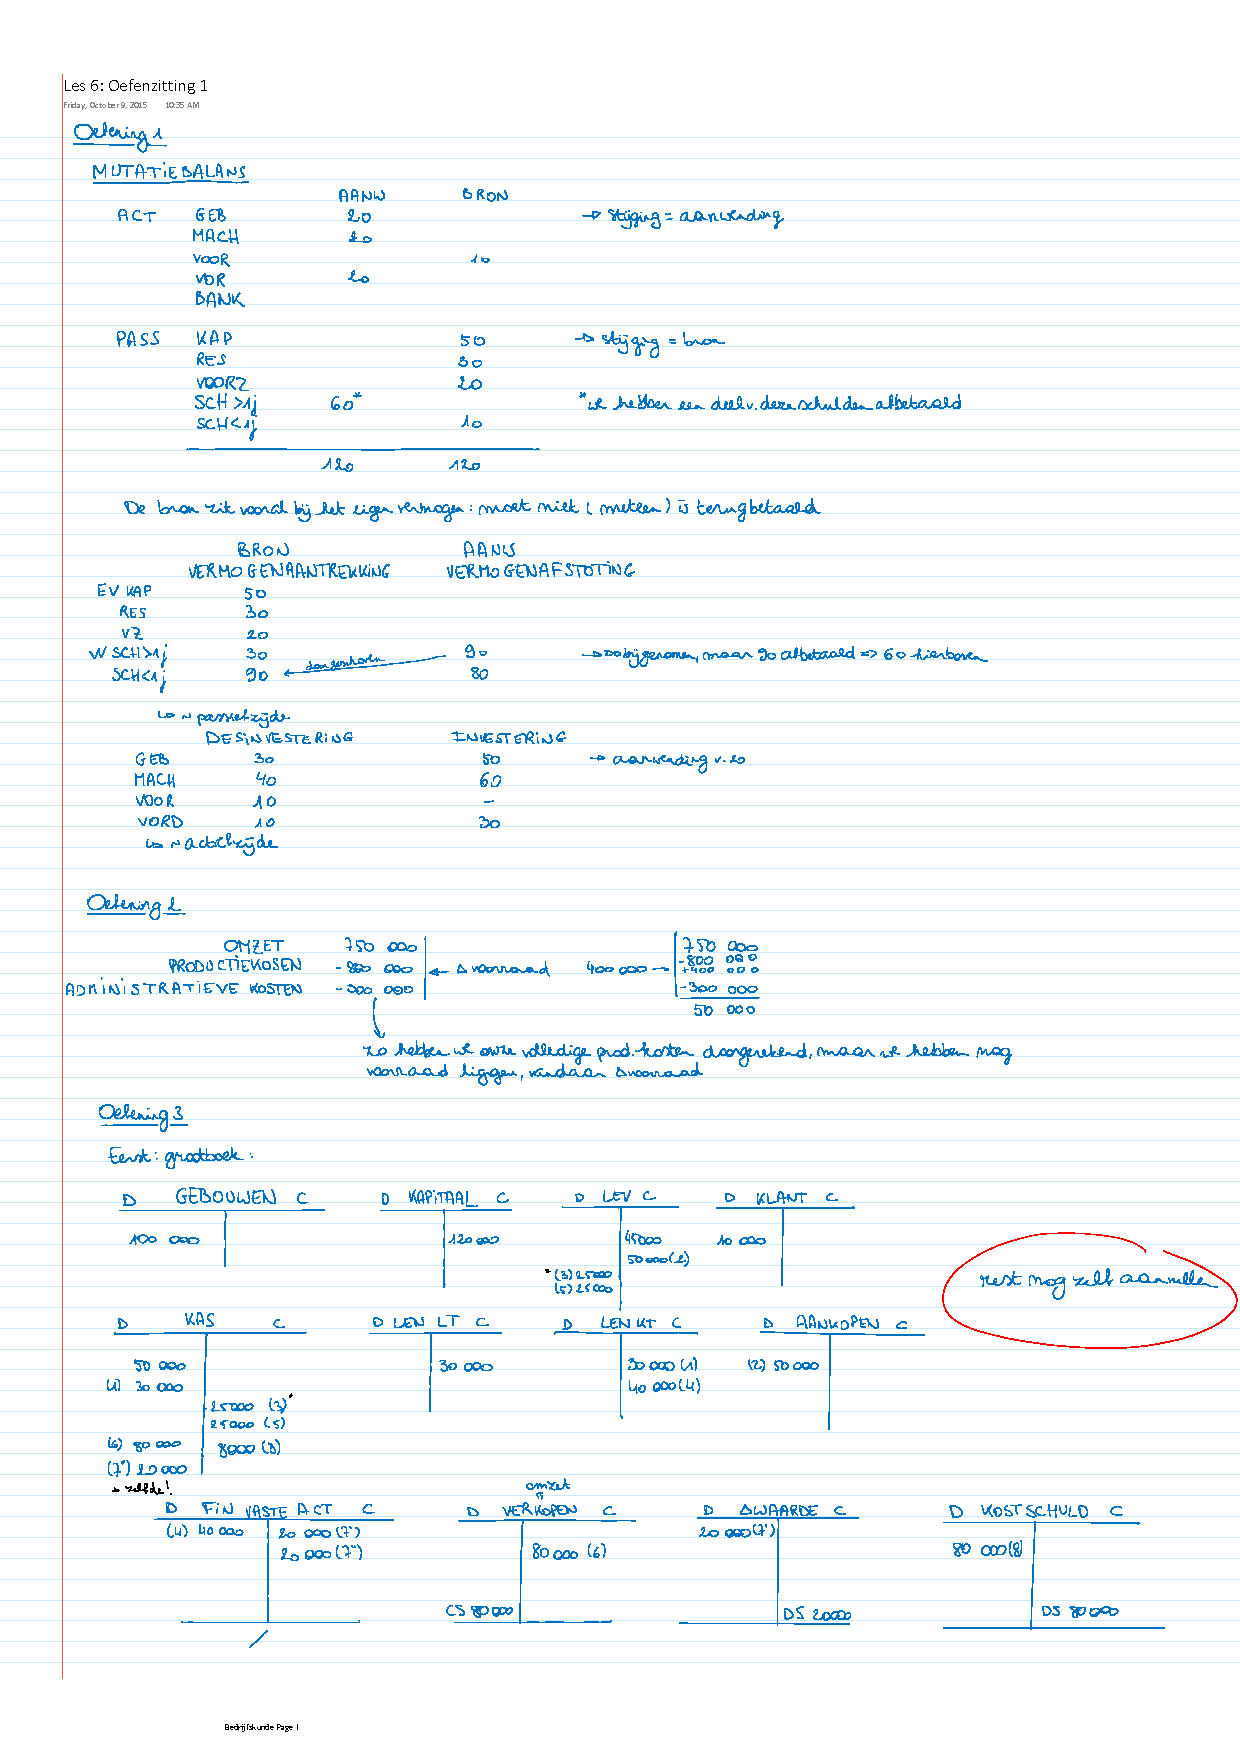
\includepdf[pages={1,2}]{Les6Oefenzitting1.pdf} 

\chapter{Les 7}

\section{Slides: 6\_Bedrijfskunde\_Kostprijssystemen}

\paragraph{Slide 31:} Je kan de kostprijs previsioneel gaan berekenen, maar dan ga je voorspellingen maken. Industri\"ele en evenredige kostprijzen worden berekend voor de toekomst: je moet schattingen maken van lonen, materialen,… en daar zal meestal een afwijking op zitten. Daarom gaaan we ook kijken naar afwijkingsanalyse. \\
Elke keer als iets afgelopen is, moet je kijken waar iets foutgelopen is als er iets fout gegaan is.

\paragraph{Slide 50:} Standaardkosten: zeer vereenvoudigd concept. We hebben de schatting en de werkelijke kost. Deze zullen zeer waarschijnlijk verschillen. We gaan het verschil uitsplitsen in de afwijking: we tellen \'e\'en keer op en trekken \'e\'en keer de elementen van elkaar af. We kunnen zo zien dat er 2 verschillen zijn: verkeerde schatting van het gebruik en verkeerde schatting van de prijs. Als dit groter is dan nul, was de werkelijke kost hoger dan geraamd. De prijsafwijking is $(p'-p)*q$, de effici\"entie-afwijking is $p(q'-q)$.

\paragraph{Slide 51:} Normale productie: de prijs die men verwachtte.

\paragraph{Slide 52 $\&$ 53:} Er zijn 150 000 stuks geproduceerd in plaats van 140 000. Het kostprijsverschil was 40. We hadden een kost van 6 000 000 geschat, maar we hadden een werkelijke kost van 6 140 000. De vraag is nu waar dat verschil vandaan komt. We gaan de formules van \textbf{Slide 51} hierop toepassen: zie Figuur \ref{les07_01}.

\begin{figure}[h!]
\centering
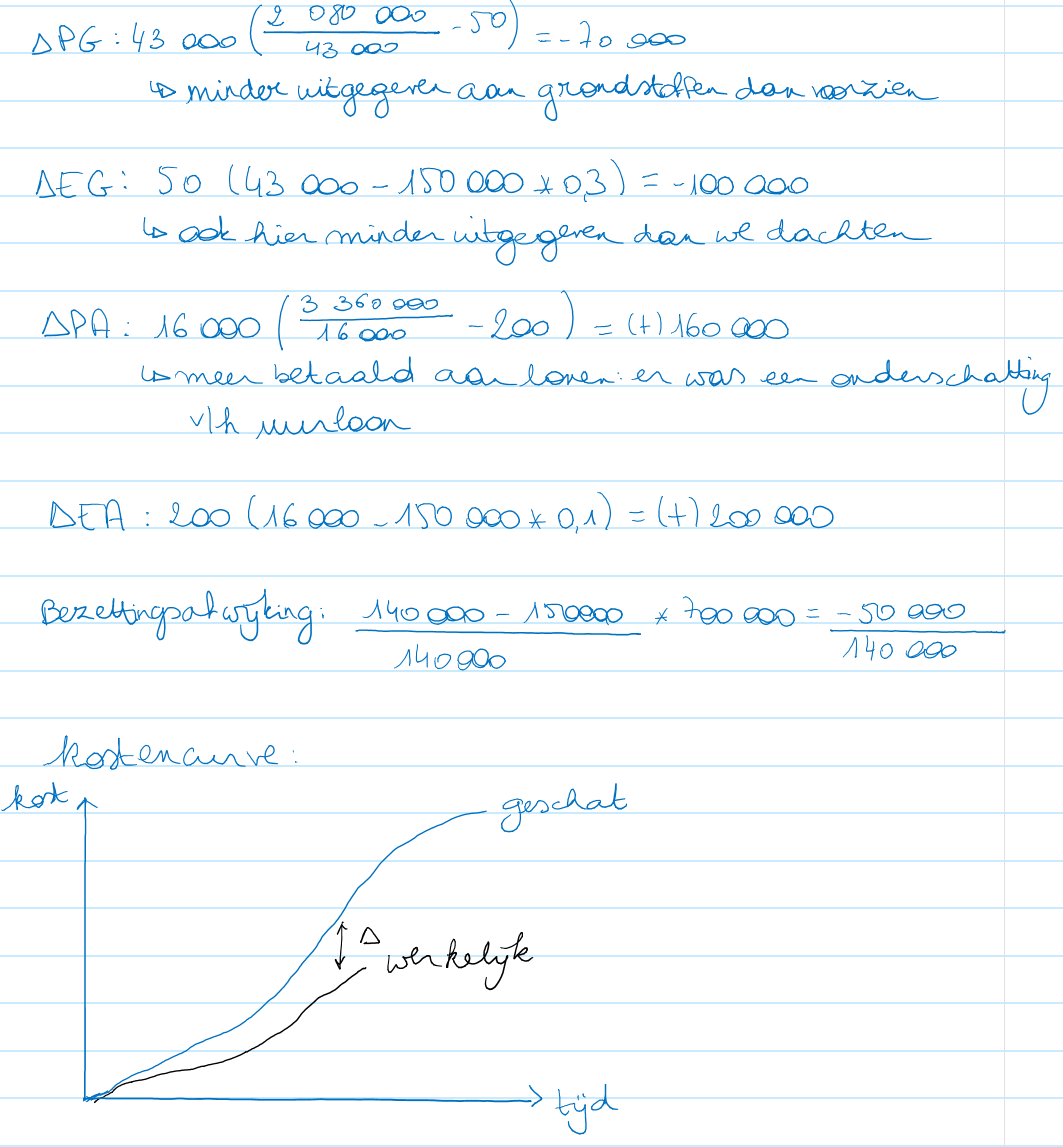
\includegraphics[width=90mm]{Les07_01.png}
\caption{Les 7 Slide 52} 
\label{les07_01}
\end{figure}

\paragraph{Slide 55:} Men besteedt meer aandacht aan overheadkosten.

\paragraph{Slide 56 e.v.:} Als we kijken naar directe arbeid: 400 000 uur per jaar en 1000 wordt gebruikt door A, dus 62 500 wordt toegewezen aan A. Er is niet nagekeken wat er met product A gebeurt. Daarom bekijjken we hetzelfde probleem opnieuw, maar we kijken wat er met A gebeurt in het magazijn.

\paragraph{Slide 58 $\&$ 59:} We delen de kost door de allocatie van de eenheid en krijgen zo de eenheidskost. Het product blijkt arbeidsintensief (de kost/eenheid is 143,75 in plaats van 62,5).

\paragraph{Slide 60:} TD-ABC: Time-Driven Activity Based Costing: men gaat kijken naar alle activiteiten en daar de tijden van noteren: elke actie wordt genoteerd als tijdsspendering aan een bepaalde actie.

\paragraph{Slide 61:} De kostenstructuur is enorm gewijzigd: vroeger waren er 95\% arbeidskosten en 5\% vaste kosten, nu is dat helemaal veranderd. Het grootste probleem is het toewijzen van overheadkosten.\\
Doordat men alle activiteiten gaat analyseren, gaat men een proces opnieuw bekijken en gaat men een aantal activiteiten volledig wijzigen.

\paragraph{Slide 63:} Target costing: reductie van de kosten door een marktonderzoek (nagaan of klanten ge\"interesseerd zijn in het product) en kijken naar de geplande verkoopprijs. We gaan hierbij kijken wat de markt bereid is te betalen voor het product. Daarna kijken we hoe we dat product kunnen opzetten (geld nodig voor materiaal, productie, distributie, levering,…). Dan zorgen dat je aan uw target kosten geraakt (verkoopprijs). Als je bepaalde zaken uitbesteedt, zorg je hierbij soms dat dit onder de target prijs gebeurt (zou moeten).\\
We zijn bezig geweest met kostprijsberekeningen waarbij we aannamen dat alles geproduceerd kon worden. In werkelijkheid gaan er bottlenecks zijn waardoor we niet alles gaan kunnen produceren en we dus een assortiment kunnen bepalen. 

\section{Slides: 7\_Economisch model}

\paragraph{Slide 3:} Wat zullen we maken en waarom?

\paragraph{Slide 4:} We willen de doelfunctie maximaliseren. In dit geval is dat het bedrijfsresultaat (R). We zullen productiehoeveelheden hebben ($q_{i}$) - de kostprijs van de verschillende producten en min de vaste kost (K).\\
We gaan capaciteitsbeperkingen krijgen, ook marktbeperkingen (saturatie van de markt).

\paragraph{Slide 5:} We hebben een doelfunctie met variabelen, kosten en opbrengsten en uiteindelijk hebben we beperkingen op machines, voorraden, beschikbare mensen,… $\rightarrow$ restricties van het aantal stuks/product.

\paragraph{Slide 6:} We kunnen relatief veel commerci\"ele gegevens bepalen. Nadelen: vrij veel variabelen en soms moeten er vereenvoudigingen gedaan worden.

\paragraph{Slide 7 e.v.:} Voorbeeld: Wat gaan we zaaien? Ma\"is of tarwe of een mengeling? Niet alleen kijken naar de opbrengst/ha, maar ook naar de opbrengst/arb. Eerst bepalen wat we als variabele gaan gebruiken. Bv Ton: $T_{t}$ $\&$ $T_{m}$: zie Figuur \ref{les07_02}.

\begin{figure}[h!]
\centering
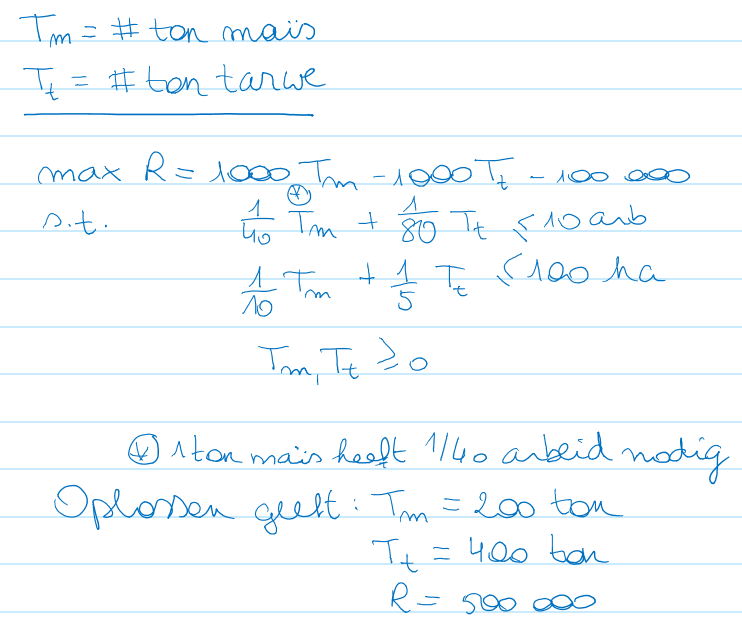
\includegraphics[width=90mm]{Les07_02.png}
\caption{Les 7 Slide 7} 
\label{les07_02}
\end{figure}

We gaan kijken naar de grafische voorstelling op \textbf{Slide 8:} beperkingen in verband met de oppervlakte en de arbeid. De ISO-margelijn is onze doelfunctie. We kunnen die doortrekken tot we in A komen, waarbij we 200 ton ma\"is krijgen en 400 ton tarwe.\\ Interessant is om te weten dat wanneer er een arbeider bijkomt, of dit interessant is of niet en wat het loon is dat eraan gegeven mag worden om geen verlies te maken. We kunnen dit berekenen door de bovenste arbeiderlijn te nemen (arbeider erbij), dan is de oplossing in B. Laten we een arbeider gaan, komen we in C terecht.\\
We kunnen ook kijken naar het duale probleem: als je je bedrijf verhuurt/verkoopt aan iemand anders, wil je minstens uw 500 000 winst terug. We krijgen: zie Figuur \ref{les07_03}.

\begin{figure}[h!]
\centering
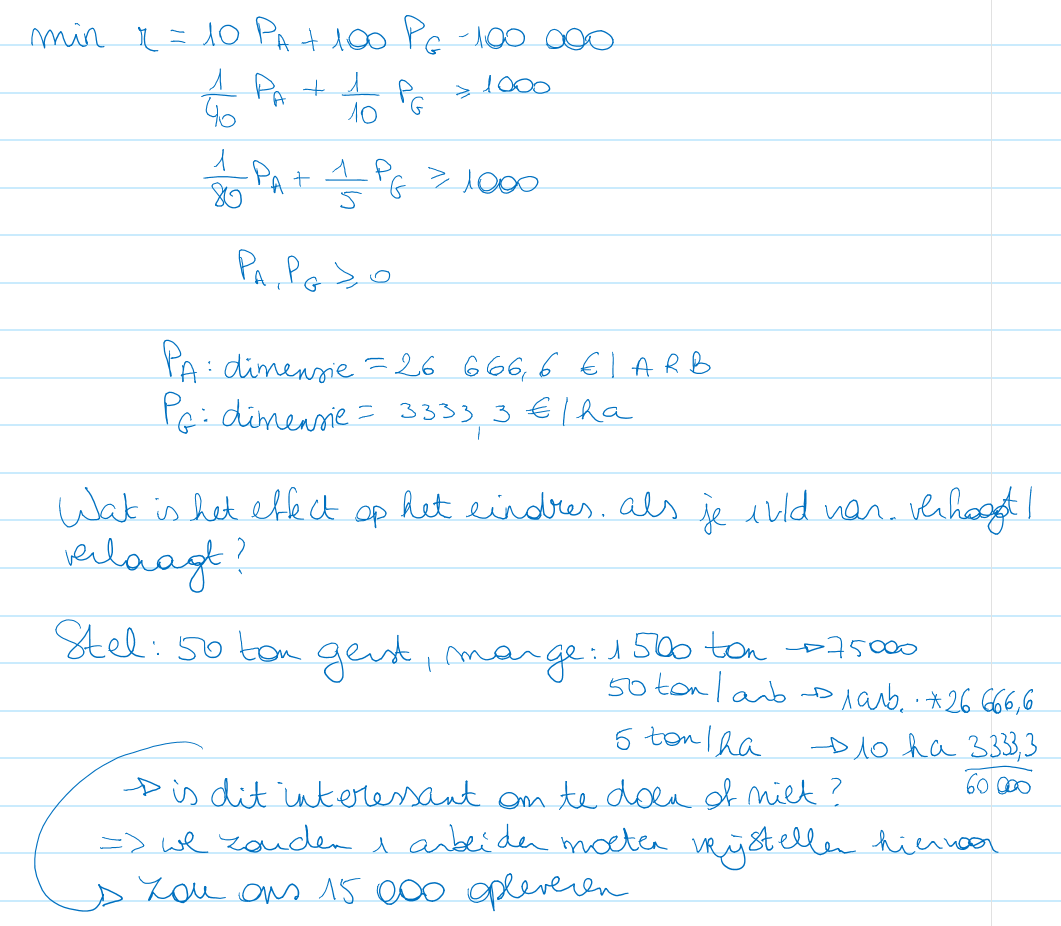
\includegraphics[width=90mm]{Les07_03.png}
\caption{Les 7 Slide 8} 
\label{les07_03}
\end{figure}

\paragraph{Slide 11:} We hebben een bedrijf dat een papiermachine heeft met een beperkte capaciteit van 1000 ton en een kost van 9/kg. Daar worden rollen geproduceerd en we hebben 2 mogelijkheden: ofwel vellen (die worden verpakt), wat ons 2/kg kost, of we pakken de rollen rechtstreeks in, met een extra kost van 1/kg. Deze worden verkocht (D) en daar hebben we verschillende markten: binnenlandse markt $\&$ export voor de vellen en binnenlandse markt $\&$ export voor de rollen. Op basis van wat hier staat kan je bepalen wat de marge per verkoopsas is. De marges staan helemaal onderaan. Je gaat zoveel mogelijk proberen zenden naar de markt met de meeste marge (dus vellen naar het binnenland). Vlak boven de marge staat het optimaal verkoopprogramma. Die 500 komt van bij het beentje van binnenland, de 200 = 700 (bij B) - 500, hierbij is dan al 700 toegewezen en voor rollen binnenland is 100 optimaal, we hebben dan nog 200 over die naar de export van rollen gaat.\\
Als we kijken naar de schaduwkosten: zie Figuur \ref{les07_04}.

\begin{figure}[h!]
\centering
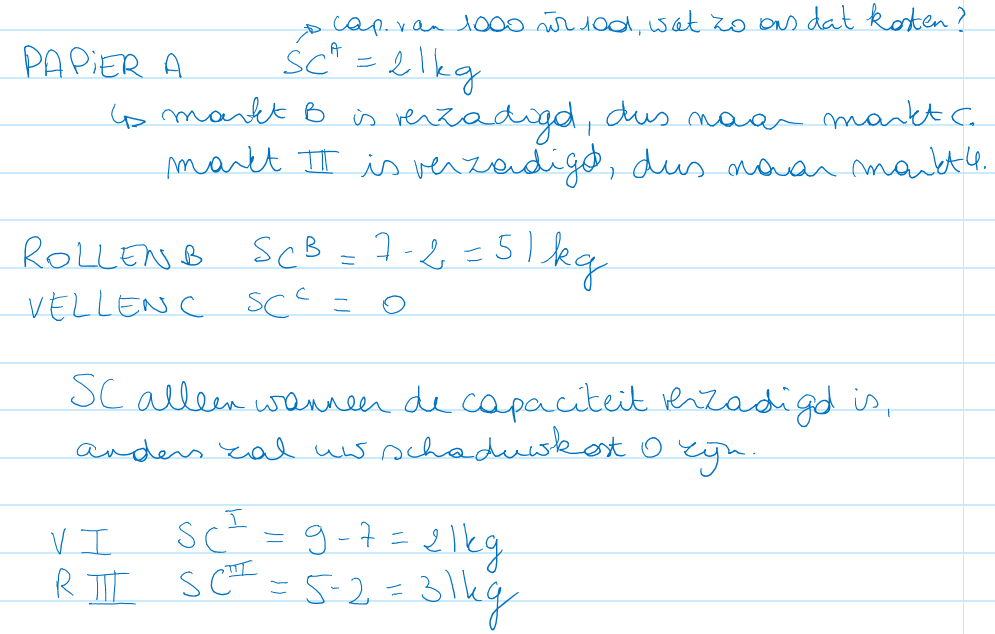
\includegraphics[width=90mm]{Les07_04.png}
\caption{Les 7 Slide 11} 
\label{les07_04}
\end{figure}

\paragraph{Slide 10:} Stel dat we een rol (\textbf{Slide 11}) willen verkopen/aankopen: welke prijs moet je daarvoor vragen? Doordat je die ene rol eruit haalt, zal je 999 rollen produceren en zal je 2 verliezen. Maar ook het inpakken van de rollen moet je inrekenen. De transferprijs is dus 9+1+2 = 12/kg. Als je de rollen verkoopt aan iemand, vraag je minstens 12, als je er een aankoopt, betaal je minstens 12.\\
Kijken we naar de transferprijs onder A (die grote pijl), dan krijgen we de schaduwkost van machine A, maar hij gaat niet meer door het inpakproces, dus we krijgen: 9+2 = 11/kg. We willen dat onze totaalverkoop qua prijs dezelfde blijft.

\paragraph{Slide 13:} Op het eerste zicht is P1 interessanter dan P2 (want 1000/stuk), maar je hebt voor P1 2 uur nodig en voor P2 maar 1 uur, wat dus neerkomt op een totaal van 500 voor P1 en 800 voor P2. P2 is dus interessanter. Als we dit in een figuur steken, krijgen we: zie Figuur \ref{les07_05}.

\begin{figure}[h!]
\centering
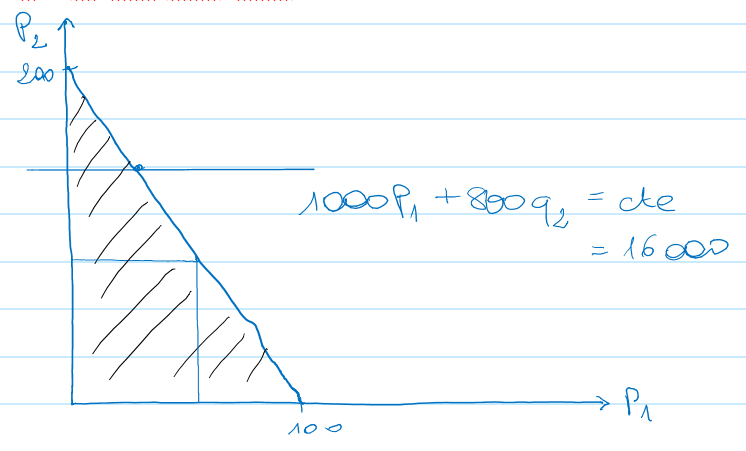
\includegraphics[width=90mm]{Les07_05.png}
\caption{Les 7 Slide 13} 
\label{les07_05}
\end{figure}

\paragraph{Slide 15:} Ander voorbeeld.\\
Conclusie: Je moet alles gaan bekijken. Als je alles kunt produceren, ga je vooral kijken naar de minimalisatie van kosten. Als je een bottleneck hebt, kun je niet alles produceren en moet je gaan uitzoeken wat voor jou het meest interessante is. Dan ga je kijken naar de marge/uur kosten. 

\chapter{Les 8}

\section{Slides: 8\_Bedrijfskunde\_Budgettering en kasplanning}

\paragraph{Slide 1:} Bedrijven moeten altijd een plan met budgetten voor de komende 5 jaar voorleggen om aan te tonen dat ze kunnen blijven bestaan, dat ze voldoende cash flow zullen kunnen genereren om te kunnen blijven bestaan.

\paragraph{Slide 3:} Elk bedrijf gaat een strategische planningscyclus hebben waarbij men bv. werkt met een tijdshorizon van 5 jaar waarbij men alle kosten zal vastleggen en ieder jaar schuift men een jaar verder door. Op het eind van het jaar gaat men analyseren wat er eventueel anders gelopen is dan voorzien en waarom.\\
Je gaat dus iedere keer een raming maken van inkomsten en uitgaven. 
Je gaat van alles inkomsten en uitgaven proberen te schatten en dit achteraf bekijken. Je moet dus kijken naar de liquiditeit en solvabiliteit (``Kunnen we de leningen, lonen,… betalen?").

\paragraph{Slide 5:} Je moet kunnen plannen en de zaken kaderen binnen de doelstellingen van het bedrijf. Je moet gaan organiseren (kan gekoppeld zijn aan de producten of aan de markten), mensen gaan motiveren en achteraf zelf controleren  en nagaan hoe alle middelen zijn toegepast.

\paragraph{Slide 6:} Gewone begroting: elk jaar een budget opstellen voor de komende 5 jaar. Investeringsbudgetten zijn eerder buitengewone begrotingen. 

\paragraph{Slide 7:} Dit is wat we willen weten: wat is onze winst, wat is onze opbrengst en wat zijn onze kosten? Het is niet zeker dat dit het eindresultaat zal zijn, vandaar dus ``(geplande)".\\
Voorraden: het opstapelen van voorraden kost ook geld, dat zit vast in uw magazijn en dat geld kan je niet gaan investeren in iets anders.

\paragraph{Slide 9:} Zie Figuur \ref{les08_01}.

\begin{figure}[h!]
\centering
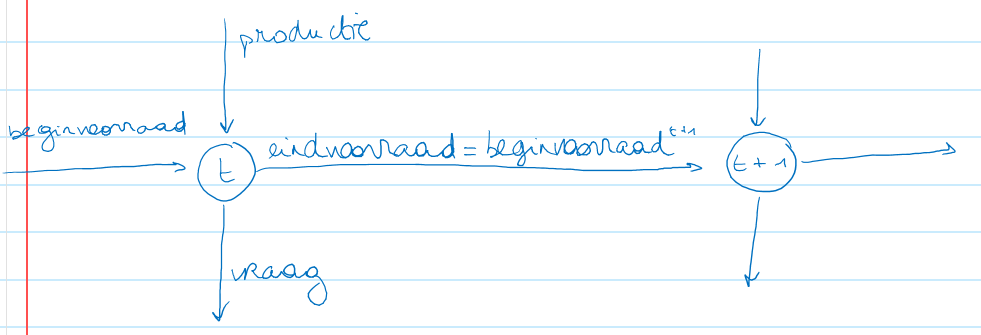
\includegraphics[width=90mm]{Les08_01.png}
\caption{Les 8 Slide 9} 
\label{les08_01}
\end{figure}

\begin{itemize}
\item Seizoenmatigheid: soms heb je pieken in de verkoop.
\item Bederfbaarheid: voorraadrotatie zo maken dat uw producten buiten zijn voor ze bedorven zijn.
\item Voorraadkosten: sommige producten moeten op speciale manieren bewaard worden (gekoeld, verwarmd,…).
\item Aankoopbeleid: kunnen we bepaalde batches aankopen en hoe groot moeten/mogen die dan zijn?
\end{itemize}

\paragraph{Slide 10:} Investeringsbudget: als je merkt dat uw capaciteit onvoldoende is om aan de vraag te voldoen, moet je investeren in nieuwe machines/mensen/… 

\paragraph{Slide 11:} Het is nodig te weten wanneer er tekorten/overschotten zijn, of sommige zaken verschoven kunnen worden, welke leningen aangegaan kunnen worden,… $\rightarrow$ previsionele resultatenrekening en balans.

\paragraph{Slide 13:} Voorbeeld: de meeste van die getallen zijn daar gewoon geplaatst (probeer ze dus niet zelf te berekenen!). Er worden soms ook afrondingen gemaakt, dus geen exacte berekeningen. Het is de bedoeling dat we proberen om zo'n tabel op te stellen. 

\paragraph{Slide 14:} Bedrijf verkoopt product X $\&$ Y, met 3 markten. Via marketingstudies checken we wat de verkopen zouden kunnen zijn in het volgende jaar (dus enkel 1 jaar bekijken, geen reeks jaren). De verkoopsaantallen zijn te zien in de onderste rij an de tabel (in kolommen van ``Eenheden"). 210 000 * 100 = 21 000 (* $10^{3}$, zie bovenaan). We gaan kijken hoe het zit met onze voorraaden. Dit zien we in de Begininventaris van de tweede tabel. Je ziet dat je niet 1 000 000 stuks gaat produceren, maar 960 000. Dit is afhankelijk van de situatie (o.a. waar in de cyclus je zit).

\paragraph{Slide 15:} Op basis daarvan kunnen we zien wat de voorraadwaarde is en de waarde per stuk (168 en 69). Een product is meestal samengesteld uit deelproducten. We gaan nog MRP (Material Requirement Planning) zien. Product X wordt samengesteld uit A, B en C: dit is de productstructuur (zie tekening op Figuur \ref{les08_02}).

\begin{figure}[h!]
\centering
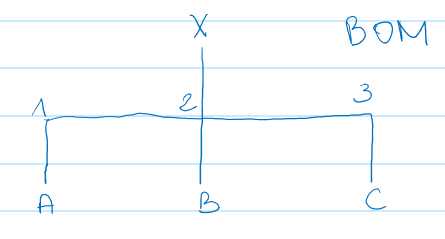
\includegraphics[width=60mm]{Les08_02.png}
\caption{Les 8 Slide 15} 
\label{les08_02}
\end{figure}

\paragraph{Slide 16:} Op basis van de voorgaande berekeningen kunnen we gaan zien hoeveel stuks we moeten gaan produceren.\\
We zien hoeveel stuks van A, B en C we nodig hebben. Hier krijgen we dan de brutobehoeften van de verschillende grondstoffen. 

\paragraph{Slide 17:} Rekening houdend met de beginvoorraad en de gewenste eindvoorraad krijg je de tabel. 

\paragraph{Slide 18:} Directe loonkosten de gelinkt zijn aan de productie. 

\paragraph{Slide 19:} Indirecte kosten: de cijfers zijn ter illustratie, niet ergens berekend. Wij zijn ge\"interesseerd in de 39 939 onderaan.

\paragraph{Slide 20:} De kostprijs die we mogen aanrekenen is kleiner dan onze aankoopprijs (70 830 vs 70 950), dit komt omdat we met voorraden zitten, we mogen die niet zomaar doorrekenen.

\paragraph{Slide 23:} Alles samenbrengen: previsionele resultatenrekening. 

\paragraph{Slide 24:} Uiteindelijk zal het zo zijn, op basis van onze productie en het feit dat het productiepark veroudert, dat we een investeringsbudget moeten samenstellen. Sommige zaken zullen over verschillende jaren lopen, je moet dat proberen opsplitsen. 

\paragraph{Slide 27:} Een budget moet opgesteld worden en je moet dit achteraf gaan controleren op verschillende facetten. Je moet ervoor zorgen dat iedereen op de hoogte is van de budgetten. Het is niet omdat iemand iets aanvraagt, dat hij/zij dat budget ook altijd krijgt, die moet zijn/haar budget eventueel ook gaan aanpassen aan wat toegewezen wordt. 

\paragraph{Slide 29:} Interpretatie van een aantal zaken.

\paragraph{Slide 30:} We gaan kijken naar de afwijking van het gebudgetteerde bedrag en de werkelijkheid. Je gebruikt bij de werkelijke productie ook 1875 omdat dat het aantal is dat je werkelijk geproduceerd hebt, maar je moet wel gaan kijken naar uw voorspelde waarden (standaard materiaalverbruik en gebudgetteerde materiaalprijs). Het materiaalverbruik en de materiaalkost bleek hoger dan voorspeld. 

\paragraph{Slide 32:} 180 000 komt van 1875 * 96. 196 875 komt van 1875 * 105. Als we effici\"ent waren geweest, had het prijsverschil even breed geweest als ``budget bij standaardverbruik", maar nu is dat dus ``budget bij standaardverbruik" + ``effici\"entieverschil).

\paragraph{Slide 33:} Zie Figuur \ref{les08_03}.

\begin{figure}[h!]
\centering
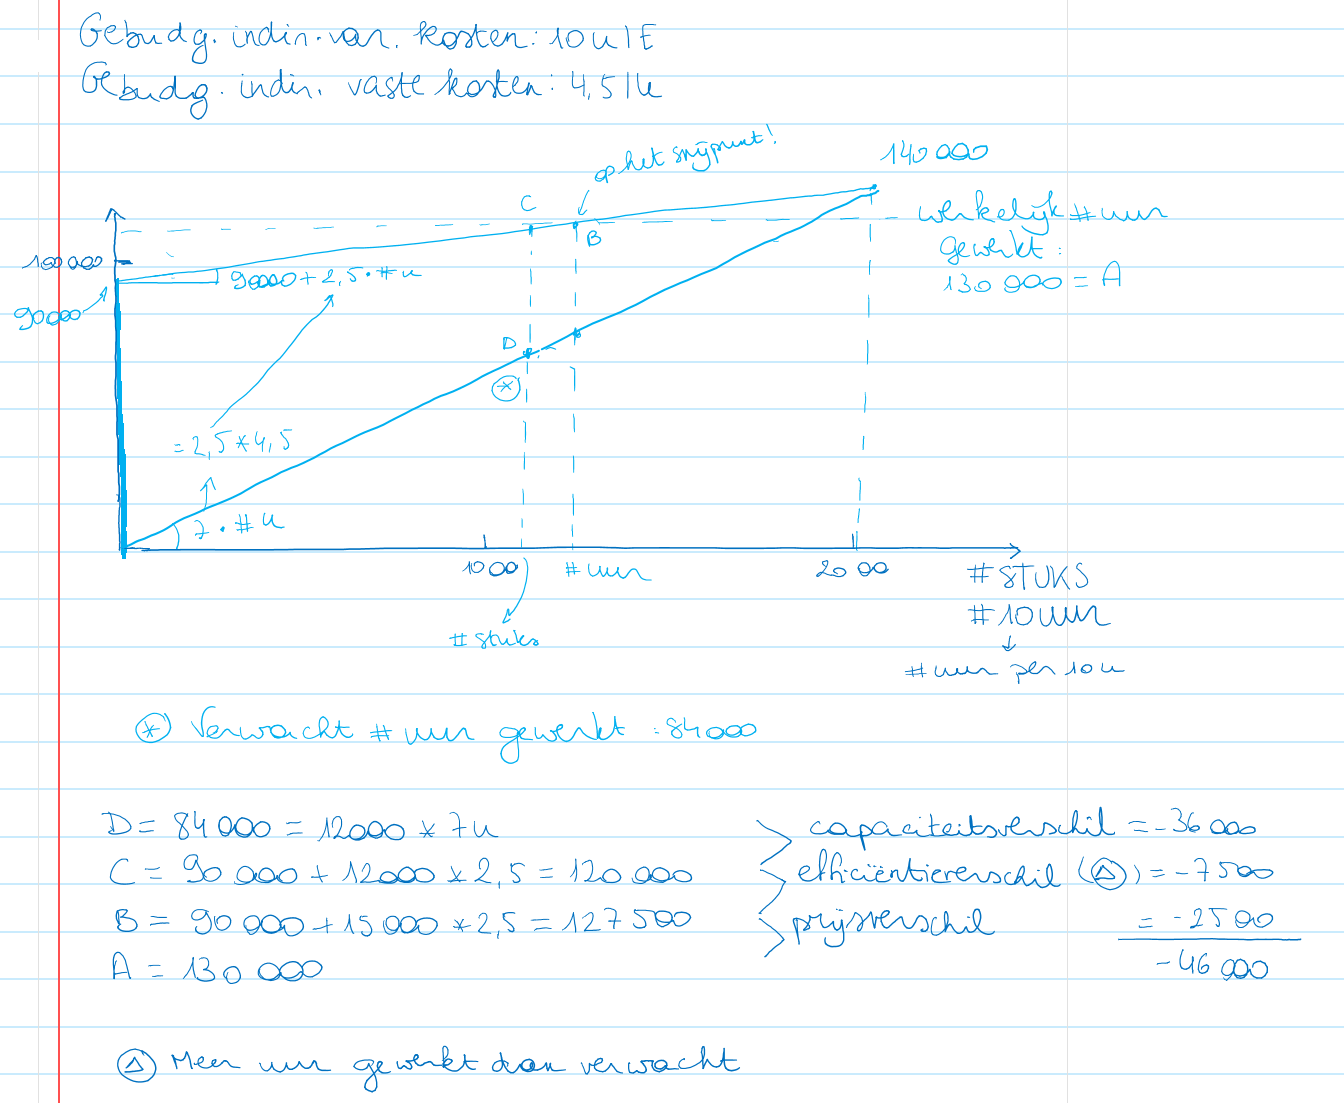
\includegraphics[width=90mm]{Les08_03.png}
\caption{Les 8 Slide 33} 
\label{les08_03}
\end{figure}

\paragraph{Slide 34:} Berekeningen bij de grafiek. Het effici\"entieverschil is puur afkomstig van variabele kosten (denk ik).
    
\section{Slides: 9\_Bedrijfskunde\_Investerings- en kostenbatenanalyse}

\paragraph{Slide 3:} Als we investeren in een nieuwe productie-eenheid (bv. fabriek), moeten we gaan nagaan waar het interessant is om te gaan investeren. 

\paragraph{Slide 4:} Het basisprincipe van een investering: we hebben een investering waarbij we ee bepaald bedrag uitgeven op een bepaald tijdstip en we hopen achteraf dat we geld extra zullen binnenkrijgen. Dat geld komt dan over een bepaalde tijdsperiode binnen, afhankelijk van de duur van onze investering. Op die manier genereer je bepaalde kasstromen. Je moet zorgen dat uw binnenkomend geld voldoende groot is om uw investering te compenseren.

\paragraph{Slide 5:}
\begin{itemize} 
\item Vervangingsprobleem: het systeem is fysisch verouderd (werkt bv. niet meer). 
\item Moderniseringsprobleem: machine kan niet meer mee.
\item Expansieprobleem: meestal wanneer je een nieuw product op de markt brengt en de markt groeit of met dalende marktvraag omgaan.
\item Strategisch probleem: nieuwe eenheden plaatsen op nieuwe locaties.
\end{itemize}

\paragraph{Slide 6:}
\begin{itemize}
\item Fysische levensduur: verouderde machines.
\item Economische levensduur: als uw product goedkoper gemaakt kan worden.
\item Productlevensduur: als uw product na 3 jaar verouderd is, ga je niet voor 10 jaar investeren in dat product, maar maar voor 3 jaar.
\item Fiscale levensduur: afschrijvingen.
\end{itemize}
Als je projecten gaat vergelijken met elkaar, moeten dat gelijkwaardige projecten zijn (project dat 2 jaar duur vs een project dat 5 jaar duurt). \\
Uitgavepatroon: alle investeringsonkosten moeten daarin gerekend worden. Je moet kijken naar alle kosten zodanig dat uw installatie kan werken.

\paragraph{Slide 7:} Kasstroom: inkomsten en uitgaven per periode (kunnen vari\"eren per periode), we krijgen dan de bruto kasstroom. Daarvan gaan we de afschrijvingen aftrekken, zo krijgen we de belastbare winst waarvan we de belastingen moeten betalen, waarop we de winst na belastingen krijgen. Daarna tellen we er de afschrijvingen opnieuw bij op (soort recuperatie die je mag doen door minder belastingen te betalen. Je moet die afschrijvingen niet nog eens betalen want dan zou je 2 keer betalen). \textcolor{red}{Als je afschrijvingen ziet als kasstromen op het examen, ben je gebuisd voor die vraag.}

\paragraph{Slide 8:} Het is belangrijk om de juiste kosten te kennen. Kern van de zaak is dat je alles wilt omzetten in geld.

\paragraph{Slide 9:}
\begin{itemize}
\item Samengestelde interesten: veronderstel dat we ergens een bepaald kapitaal p hebben dat we beleggen. Als we dat beleggen aan een bepaalde interest, wil dat zeggen dat na 1 periode het kapitaal gelijk is aan P + Pi. Als je dat bedrag dan opnieuw belegt, dan zal P vermenigvuldigd worden met i, maar uw interest ook. Het kapitaal waarmee we startten zal dus gelijk zijn aan $F = P(1+i)^{n}$ als je alles hebt laten staan.
\end{itemize}
\paragraph{Slide 10:} Bij hoge interestvoeten zie je dat je niet lineair mag denken, bij kleine interestvoeten zal de geschatte en de werkelijke opbrengst ongeveer gelijklopen.

\paragraph{Slide 11:} De meest linkse kolom is het aantal periodes. Bovenaan vind je dan telkens het aantal percentages terug. Je ziet dan na hoeveel periodes je hoeveel zal hebben.

\paragraph{Slide 13:} We gaan normaal alles proberen terugbrengen naar het ``nu"-moment: naar de waarden die nu geldig zijn. Daarom spreken we over actualisatie. 

\paragraph{Slide 15 $\&$ 16:} Huidige waarde van 1 Euro. Let op dat er gesproken is over periodes en niet over jaren. Het kan zijn dat men over trimesters spreekt en niet over jaren.

\paragraph{Slide 17:} We zullen niet 1 bedrag hebben dat binnenkomt, maar dat zal verspreid zijn over de horizon. Dit kunnen uiteraard ook negatieve waarden zijn. Je moet uiteindelijk altijd vergelijken met het nulmoment.

\paragraph{Slide 18:} We kunnen de gegeven vraag gaan berekenen: zie Figuur \ref{les08_04}.

\begin{figure}[h!]
\centering
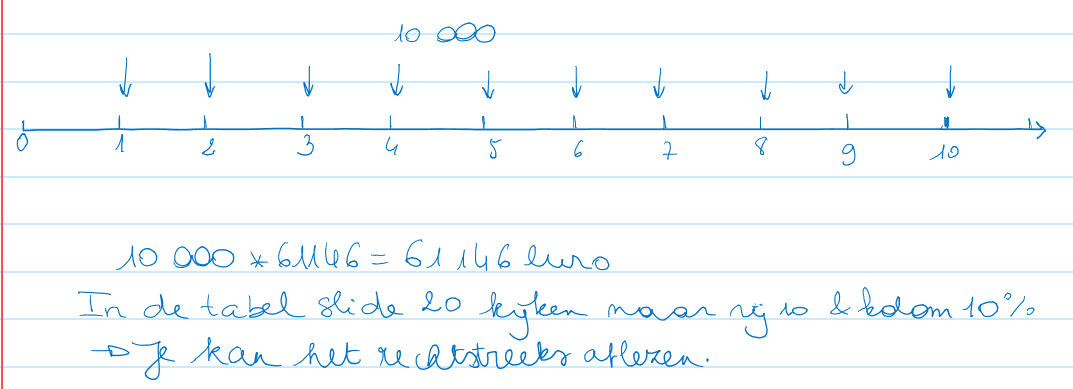
\includegraphics[width=90mm]{Les08_04.png}
\caption{Les 8 Slide 18} 
\label{les08_04}
\end{figure}

\paragraph{Slide 21:} Banklening van 100 000 en je hebt een trimesteri\"ele rentevoet van 4\%. De terugbetalingen gebeuren altijd op een specifiek moment. We hebben n = 5 en I = 4\%. Kijken we in onze tabel op \textbf{Slide 19} (rij 5, kolom van 4\%), krijgen we: A*4,4518 = 100 000 $\Rightarrow$ A = 22 463.\\
Hoe wordt dat nu allemaal uitgesplitst? Zie Figuur \ref{les08_05}.

\begin{figure}[h!]
\centering
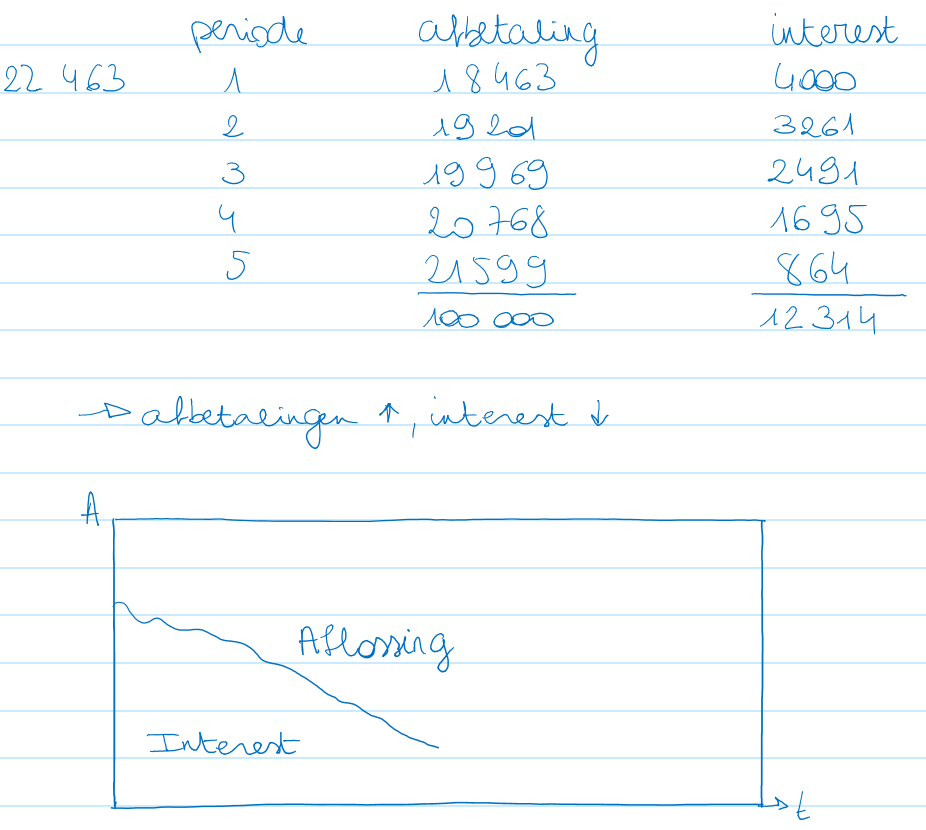
\includegraphics[width=90mm]{Les08_05.png}
\caption{Les 8 Slide 21} 
\label{les08_05}
\end{figure}

\paragraph{Slide 22:} Overgeslagen.

\paragraph{Slide 23:} Zie Figuur \ref{les08_06}.

\begin{figure}[h!]
\centering
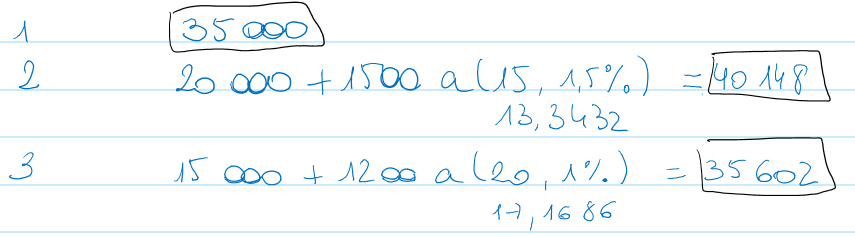
\includegraphics[width=90mm]{Les08_06.png}
\caption{Les 8 Slide 23} 
\label{les08_06}
\end{figure}

Niet zomaar voor 2 of 3 kiezen, je moet nog steeds 20 000 investeren! De eerste optie is duidelijk de goedkoopste.

\chapter{Les 9}

\section{Slides: 9\_Bedrijfskunde\_Investerings- en kostenbatenanalyse}

\paragraph{Slide 24:} We weten hoe snel een investering wordt terugbetaald. Op de horizontale as hebben we de tijdshorizon, op de verticale as hebben we een overzicht van de kasstromen. Op tijdstip 0 hebben we ons investeringsbedrag gehad. Het is de bedoeling dat zo'n investering geld opbrengt in de toekomst. Wanneer we alles cumulatief uitzetten, is het de bedoeling dat de positieve kasstromen groter worden dan de negatieve zodat we boven 0 uitkomen, anders is de investering niet interessant. Bij curve 1 komen we relatief snel naar boven en hebben we een relatief korte terugbetalingstermijn. Bij de tweede is dat minder snel. Het eerste project is dus interessanter dan het tweede. Dit heeft een aantal nadelen: we zijn kortzichtig want we kijken alleen naar de eerste inkomsten en niet naar latere inkomensten, we willen ons geld zo snel mogelijk opnieuw recupereren. We houden geen rekening met achterliggende inkomsten.\\
Curve 2 toont mooie kasstromen later, maar je kan de verre toekomst niet voorspellen. In de nabije toekomst kan je veel beter voorspeleln. Daarom kijkt men voornamelijk naar hoe snel de investering wordt terugbetaald.

\paragraph{Slide 25:} Men gaat kijken naar de netto waarde. We kijken naar de kasstroom teruggebracht naar het nu-moment. We gaan kijken naar de inkomsten (R: revenue) en uitgaven (E: expenses). Daar nemen we de netto waarde van en passen we die aan met de juiste actualisatievoet om die terug te brengen naar het nu-moment. Naarmate k stijgt, wordt de factor in de noemer groter en gaat de waarde dalen in het nu-moment.\\
Meestal kijkt men naar de netto huidige waarde: huidige waarde - investeringsbedrag. Een investering is interessant wanneer de netto huidige waarde positief is. Als we moeten kiezen tussen 2 projecten, kiezen we dat project met de grootste netto huidige waarde. NHW(A) = 10 000 NHW(B) = 8000. Je zou intu\"itief voor A kiezen, maar je weet hier niets over de tijd. Je moet ook kijken naar het investeringsbedrag: stel: $I_{0A}$ = 1 000 000 en $I_{0B}$ = 250 000. Bij B heb je nog 750 000 over die ook iets zullen opbrengen. Je moet altijd alles dus op de juiste manier analyseren en bekijken.

\paragraph{Slide 26:} Meest gebruikt: houdt rekening met beiden. We hebben gemerkt dat 2 verschillende regels 2 verschillende rangorders kunnen geven. Je moet alles dus altijd grondig analyseren en bekijken.

\paragraph{Slide 27:} Inwendige rendementsgraad: als we ergens onze NHW plaatsen in functie van de interestvoet, dan gaan we die berekenen voor een bepaalde i. hopelijk vinden we dan ergens een positieve waarde. Laten we die i vari\"eren, zal die waarde ook mee vari\"eren. Als we werken met een systeem waarbij we 1 uitgave hebben en voor de rest allemaal inkomsten, wat zal er dan gebeuren als de i kleiner wordt, wat gebeurt er dan met de NHW? Als i kleiner wordt, zal de waarde stijgen. Zie Figuur \ref{les09_01}.

\begin{figure}[h!]
\centering
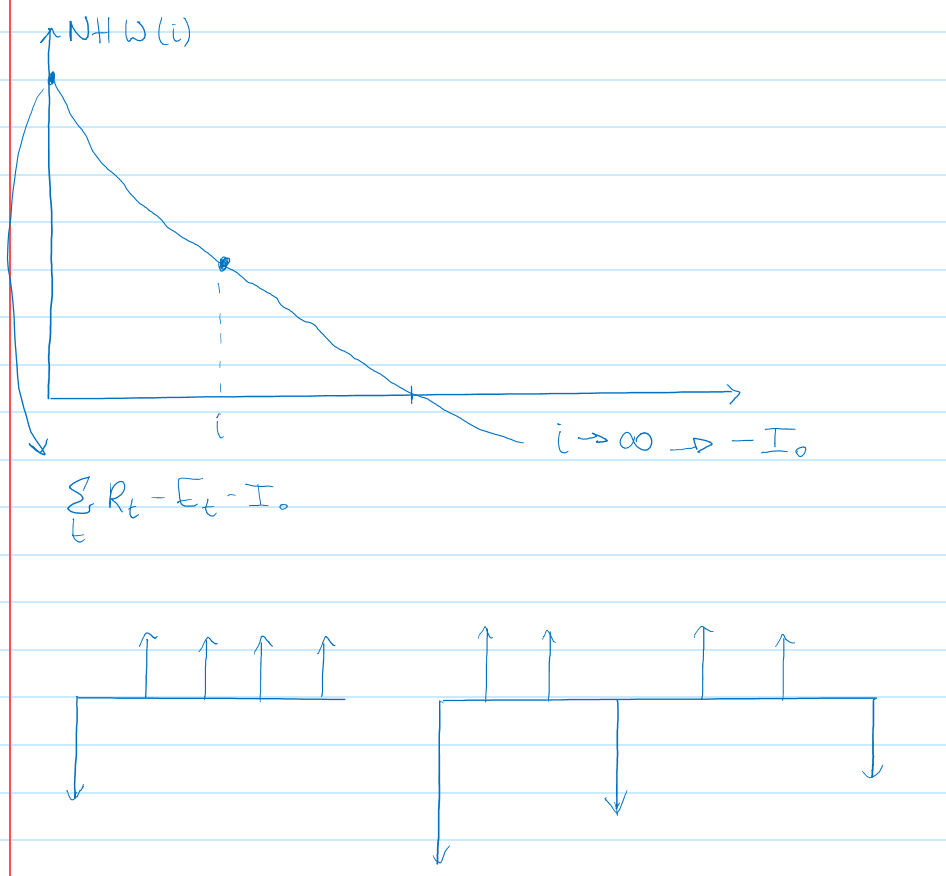
\includegraphics[width=90mm]{Les09_01.png}
\caption{Les 9 Slide 27} 
\label{les09_01}
\end{figure}

\paragraph{Slide 29:} 1 is interessanter (via de inwendige rendementsgraad) dan 2, terwijl we volgens de NHW net het omgekeerde vinden. Je moet dan gaan nagaan hoe het juist zit. 

\paragraph{Slide 30:} Zie Figuur \ref{les09_02}.

\begin{figure}[h!]
\centering
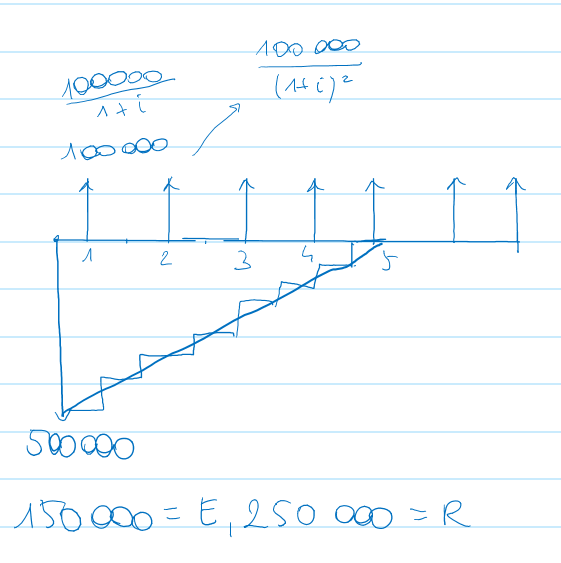
\includegraphics[width=90mm]{Les09_02.png}
\caption{Les 9 Slide 30} 
\label{les09_02}
\end{figure}

\paragraph{Slide 31:} Zie Figuur \ref{les09_03}.

\begin{figure}[h!]
\centering
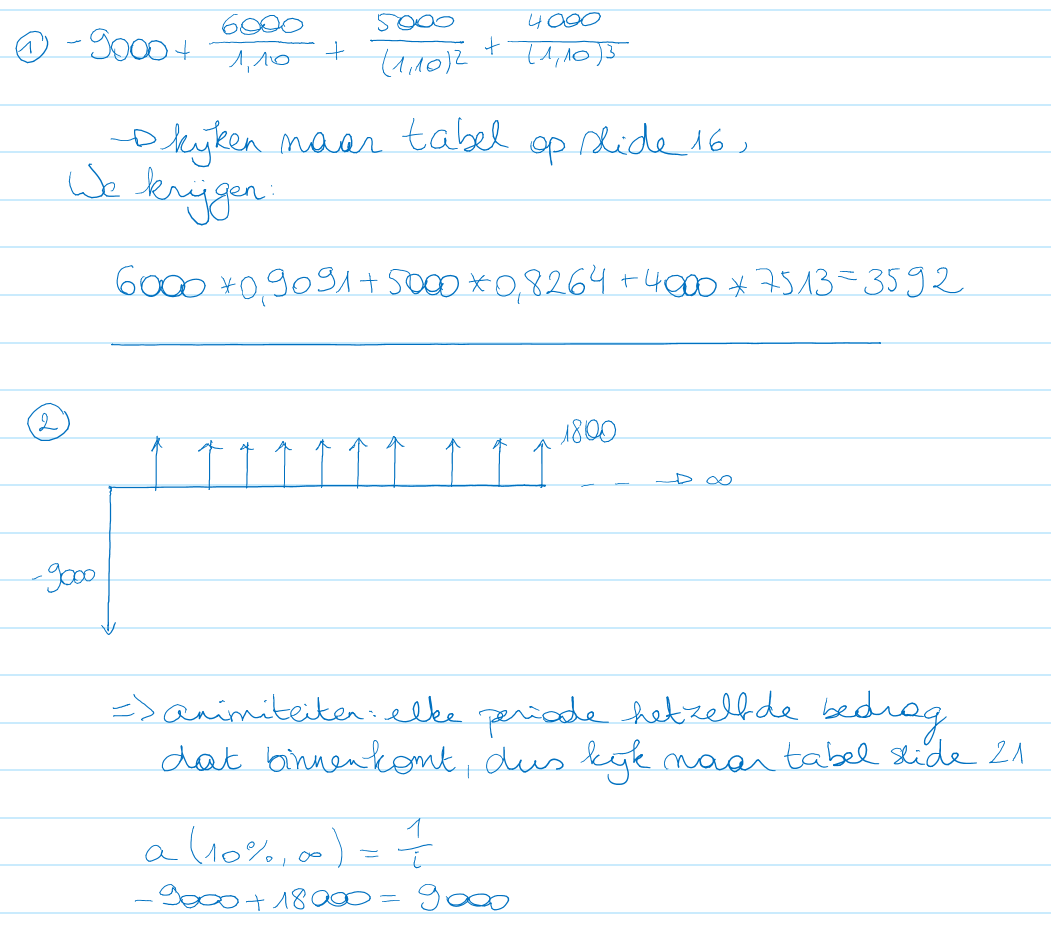
\includegraphics[width=90mm]{Les09_03.png}
\caption{Les 9 Slide 31} 
\label{les09_03}
\end{figure}

\paragraph{Slide 32:} Let op: lichte aanpassingen tegenover het boek. We gaan maar 500 000 afschrijven en geen 600 000. Zie Figuur \ref{les09_04} $\&$ \ref{les09_05}.

\begin{figure}[h!]
\centering
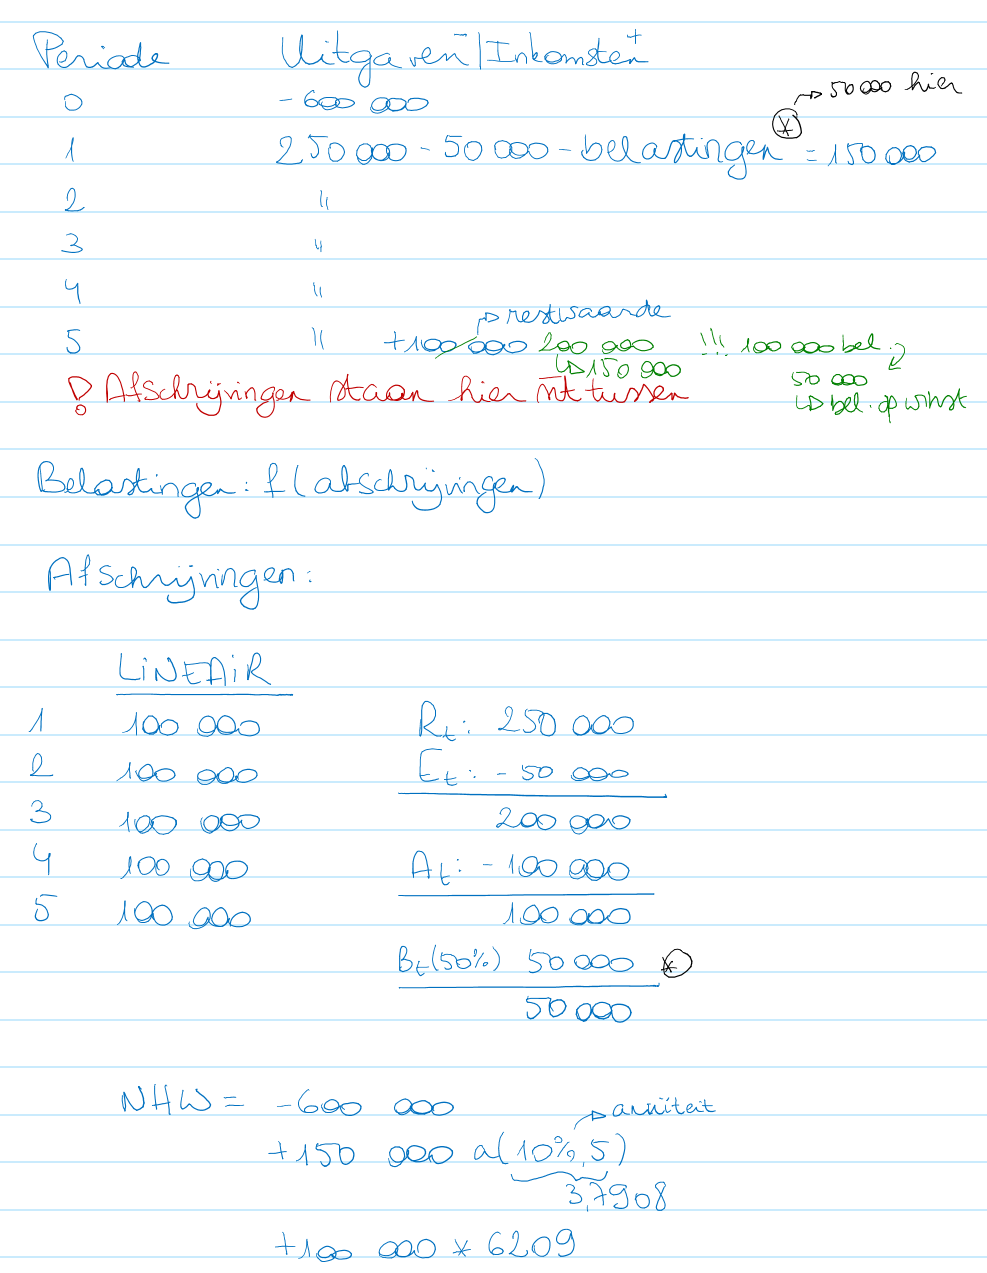
\includegraphics[width=90mm]{Les09_04.png}
\caption{Les 9 Slide 32} 
\label{les09_04}
\end{figure}

\begin{figure}[h!]
\centering
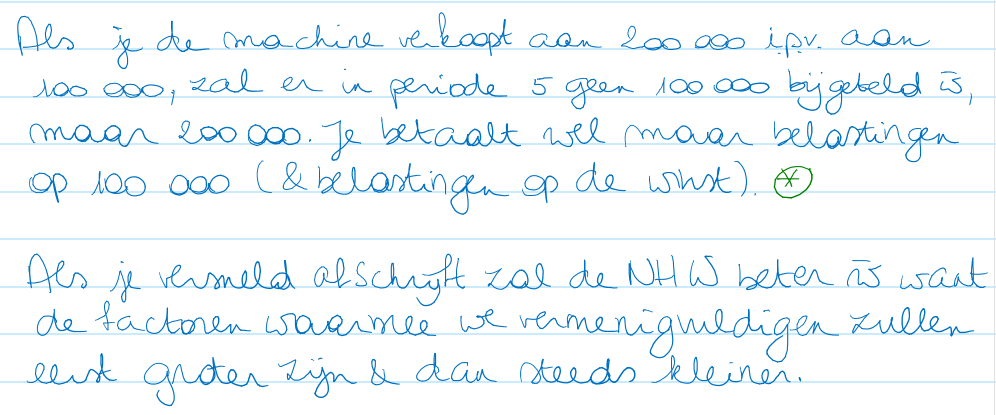
\includegraphics[width=90mm]{Les09_05.png}
\caption{Les 9 Slide 32} 
\label{les09_05}
\end{figure}

\paragraph{Slide 33:} Project z zal het interessantst zijn.

\paragraph{Slide 34:} Hier moet je ook rekening mee houden, kan uw resultaten ook be\"invloeden. Men gaat normaal ook nooit werken met 1 interestvoet, maar met verschillende om te kijken wat de variatie is, want als je curve steiler is, zal een variatie in i een zeer groot effect hebben en wanneer ze minder steil is, zal een variatie in i nauwelijks effect hebben.

\paragraph{Slide 36:} Soort screening: kijken of een project aan een bepaalde eis voldoet. Naarmate de `qualifies' stijgt, zal het project interessanter zijn.

\paragraph{Slide 37:} Een meer genuanceerd antwoord.

\paragraph{Slide 35:} Ook meer uitgebreide technieken.

\paragraph{Slide 38:} De beoordeling van \textbf{Slide 37} visueel voorgesteld. B scoort overal slechter dan A (tenzij gelijk). Je zal dus nooit B nemen als je A kan nemen. Bij C is het genuanceerder, daar hangt het er vanaf aan welk criterium je meer waarde hecht.

\paragraph{Slide 39:} Gradaties en gewichten. Het grote probleem hiermee is dat men elk resultaat kan bekomen wat men wil. Dit mag niet ingevuld worden door 1 persoon, maar door verschillende waarbij duidelijk te zien is wie wat doet.

\section{Slides: 10\_Bedrijfskunde\_Voorspellingstechnieken}

\paragraph{Slide 3:} Hoeveel banden gaan we maken in augustus? Is dit een makkelijke vraag? Bandenbedrijven zullen dit vrij goed kunnen schatten op basis van de verkoop van wagens etc. Normaal heb je eerst een order dat binnenkomt voor de aankoop van wagens en op basis daarvan zullen ze gaan voorspellen hoeveel banden er gemaakt moeten worden.

\paragraph{Slide 5:} We moeten rekening houden met het tijdsschema: afhankelijk van of we op korte of lange termijn voorspellen, gaan we op een ander niveau werken. Werken we op lange termijn, dan gaan we geaggregeerd werken. Bij lange termijn gaat men kijken naar capaciteitsbehoeften, bij intermediate gaat men kijken naar mensen en bij short gaat men kijken naar shifts.

\paragraph{Slide 6:} Voorspellingstechnieken zijn meestal fout: zie ook \textbf{Slide 7}. Als we bezig zijn met voorspellingen, moet je ervoor zorgen dat je niet eender welk getal krijgt, maar ook redenen geven waarom je dingen denkt. Het zou ook neergeschreven moeten zijn zodat men niet zomaar van mening kan veranderen. Geaggregeerde voorspellingen zijn vrij eenvoudig. De eerste jaren die we voorspellen zijn meestal vrij nauwkeurig, daarna wordt het minder nauwkeurig. \\
Je moet ook altijd proberen alle mogelijke informatie te gebruiken die aanwezig is. 

\paragraph{Slide 8:} Een goede forecast moet:
\begin{itemize}
\item op tijd zijn: als je achteraf voorspellingen doet, is het natuurlijk makkelijk;
\item zo nauwkeurig mogelijk zijn;
\item betrouwbaar zijn;
\item betekenisvolle eenheden hebben;
\item opgeschreven zijn;
\item begrijpbaar zijn voor eventuele opvolgers.
\end{itemize}

\paragraph{Slide 9:} Je moet beginnen met het identificeren van het probleem. Je moet voorspellingen doen voor zaken die nuttig en interessant zijn. Je moet zorgen dat je het probleem kent.

\paragraph{Slide 10:} Je moet kijken naar de impact en of het een eenmalige beslissing is, of een beslissing die regelmatig terugkomt. Je moet iets maken dat wel degelijk werkt als het terugkerend is, bij eenmalig kan je eventueel anders werken.

\paragraph{Slide 11:} We gaan kijken of er data beschikbaar is. Als die beschikbaar is, moet je die gaan analyseren. Dit is een heel belangrijke stap. Je moet ook gaan kijken of uw data al dan niet kwantitatief is. Als ze kwantitatief zijn, kan je kijken of er causale factoren zijn (bv. verkoop van wagens $\rightarrow$ verkoop van banden).
Als er geen causale factoren zijn, gaan we tijdsanalyses doen. Als men geen data heeft, gaat men die moeten collecteren. Deze kunnen kwantitatief zijn. Als de gegevens kwalitatief zijn, gaat men ook anders te werk.

\paragraph{Slide 12:} Je moet het probleem snappen, weten wat er gebeurt. Je moet proberen alle mogelijke extra informatie erbij te krijgen. Het is belangrijk dat je begrijpt wat er juist aan het gebeuren is. Bv. wat is het gevolg van de blauwe curve? Je weet het niet, want je weet niet waarover het gaat!

\begin{figure}[h!]
\centering
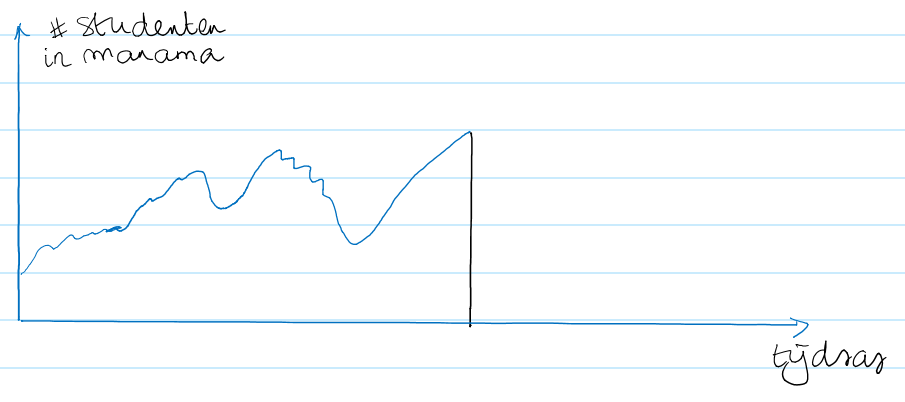
\includegraphics[width=90mm]{Les09_06.png}
\caption{Les 9 Slide 12} 
\label{les09_06}
\end{figure}

Met de zwarte informatie (niet de vervollediging van de grafiek) weet je meer. Het is hier zichtbaar hoe goed de markt is om een manama te doen. Uiteindelijk worden ze niet meer gesubsidi\"eerd, dus wordt deze uiteindelijk afgeschaft. Dit kon je niet weten/voorspellen vanuit de blauwe curve alleen, zonder info.

\paragraph{Slide 13:} Als je een curve analyseert, moet je dus rekening houden met alle gegevens die beschikbaar zijn. Maak ook altijd figuren, want het oog kan dingen afleiden die anders niet duidelijk zouden worden.

\paragraph{Slide 14:} Wanneer we zaken analyseren, gaan we een onderscheid maken tussen verschillende soorten processen. In deze slide kan je zien dat er ongeveer een constante is, waarbij we de ruis weglaten. 

\paragraph{Slide 15:} Het kan ook zijn dat we een bepaalde trendlijn hebben, of dat er een seizoensinvloed is. Het is ook mogelijk dat uw seizoensinvloed in steigende lijn gaat. 

\paragraph{Slide 17:} Je mag ``subjectief" hier niet negatief bekijken. Je kan gaan kijken op basis van verkoopsagenten. Je kan gebruik maken van enqu\^etes die je rondstuurt. 

\paragraph{Slide 18:} Een enqu\^ete is een krachtig middel, maar het moet op de juiste manier gebruikt worden. Veel zaken lopen fout omdat er te weinig aandacht besteed wordt tijdens het opzetten. Je moet een vragenreeks opstellen zodat bepaalde punten naar voren komen en de vragen die je hebt beantwoord worden. Je moet zorgen dat de vragen eenduidig opgesteld zijn. Reeds bij het opstarten moet je kijken wat voor antwoorden je gaat krijgen en hoe je die gaat verwerken. Dan pas ga je die uitvoeren. Normaal gezien zal een 10-50\% van de aangesproken mensen reageren.\\
Als je een enqu\^ete rondstuurt, moet je zien dat die in orde is, je kan moeilijk vragen om ze nog eens in te vullen omdat er iets was misgelopen. De resultaten moet je gaan analyseren en interpreteren. Het is ook fijn voor de mensen die de enqu\^ete hebben ingevuld om te weten wat de resultaten zijn.

\paragraph{Slide 20:} Expertopinie: marketingmensen bij elkaar brengen, die weten wat er met een bepaalde markt zal gebeuren. Die kunnen dan samenzitten en discussi\"eren. Zij kunnen tot conclusies komen. Er zullen altijd een aantal mensen meer naar voor komen qua input, terwijl de anderen misschien ook interessante informatie hebben.\\
Er is ook een meer formele techniek, namelijk de Delphi-methode: de experten worden niet bij elkaar geplaatst maar ze zullen vragenlijsten binnenkrijgen die ze elk apart moeten beantwoorden. Zo krijg je geen interferentie. Dan ga je voorspellingen geven. Alle antwoorden die worden binnengebracht, worden samengevat en de mensen die het hebben ingevuld krijgen hun antwoorden en het gemiddelde, zodat ze hun antwoorden kunnen motiveren of aanpassen. Dit wordt herhaald tot men tot een convergentiepunt komt.

\paragraph{Slide 21:} Voordeel: verschillende achtergronden en weinig interferentie.\\
Nadeel: neemt heel veel tijd in beslag en het kan zijn dat je geen overeenkomst bereikt.

\paragraph{Slide 22 $\&$ 23:} Voorbeeld.

\paragraph{Slide 24:} Normaal, wanneer we kijken naar het resultaat hiervan, zullen we zien dat expertopinie meestal voldoende is. De Delphi-methode is tijdsverslindend en duur (je moet al die experts betalen). Bij ``gewone" correspondenten kan het goedkoper/gratis zijn, maar het kan langer duren vooraleer je antwoord hebt. 

\paragraph{Slide 25:} Als we kwantitatieve data hebben, zullen we ofwel van causale modellen gebruik maken, ofwel van tijdsreeksen. Bovenste zijn causale modellen, onderste zijn tijdsreeksen.

\chapter{Les 10: Oefenzitting 2}
Zie volgende pagina voor handgeschreven nota's.

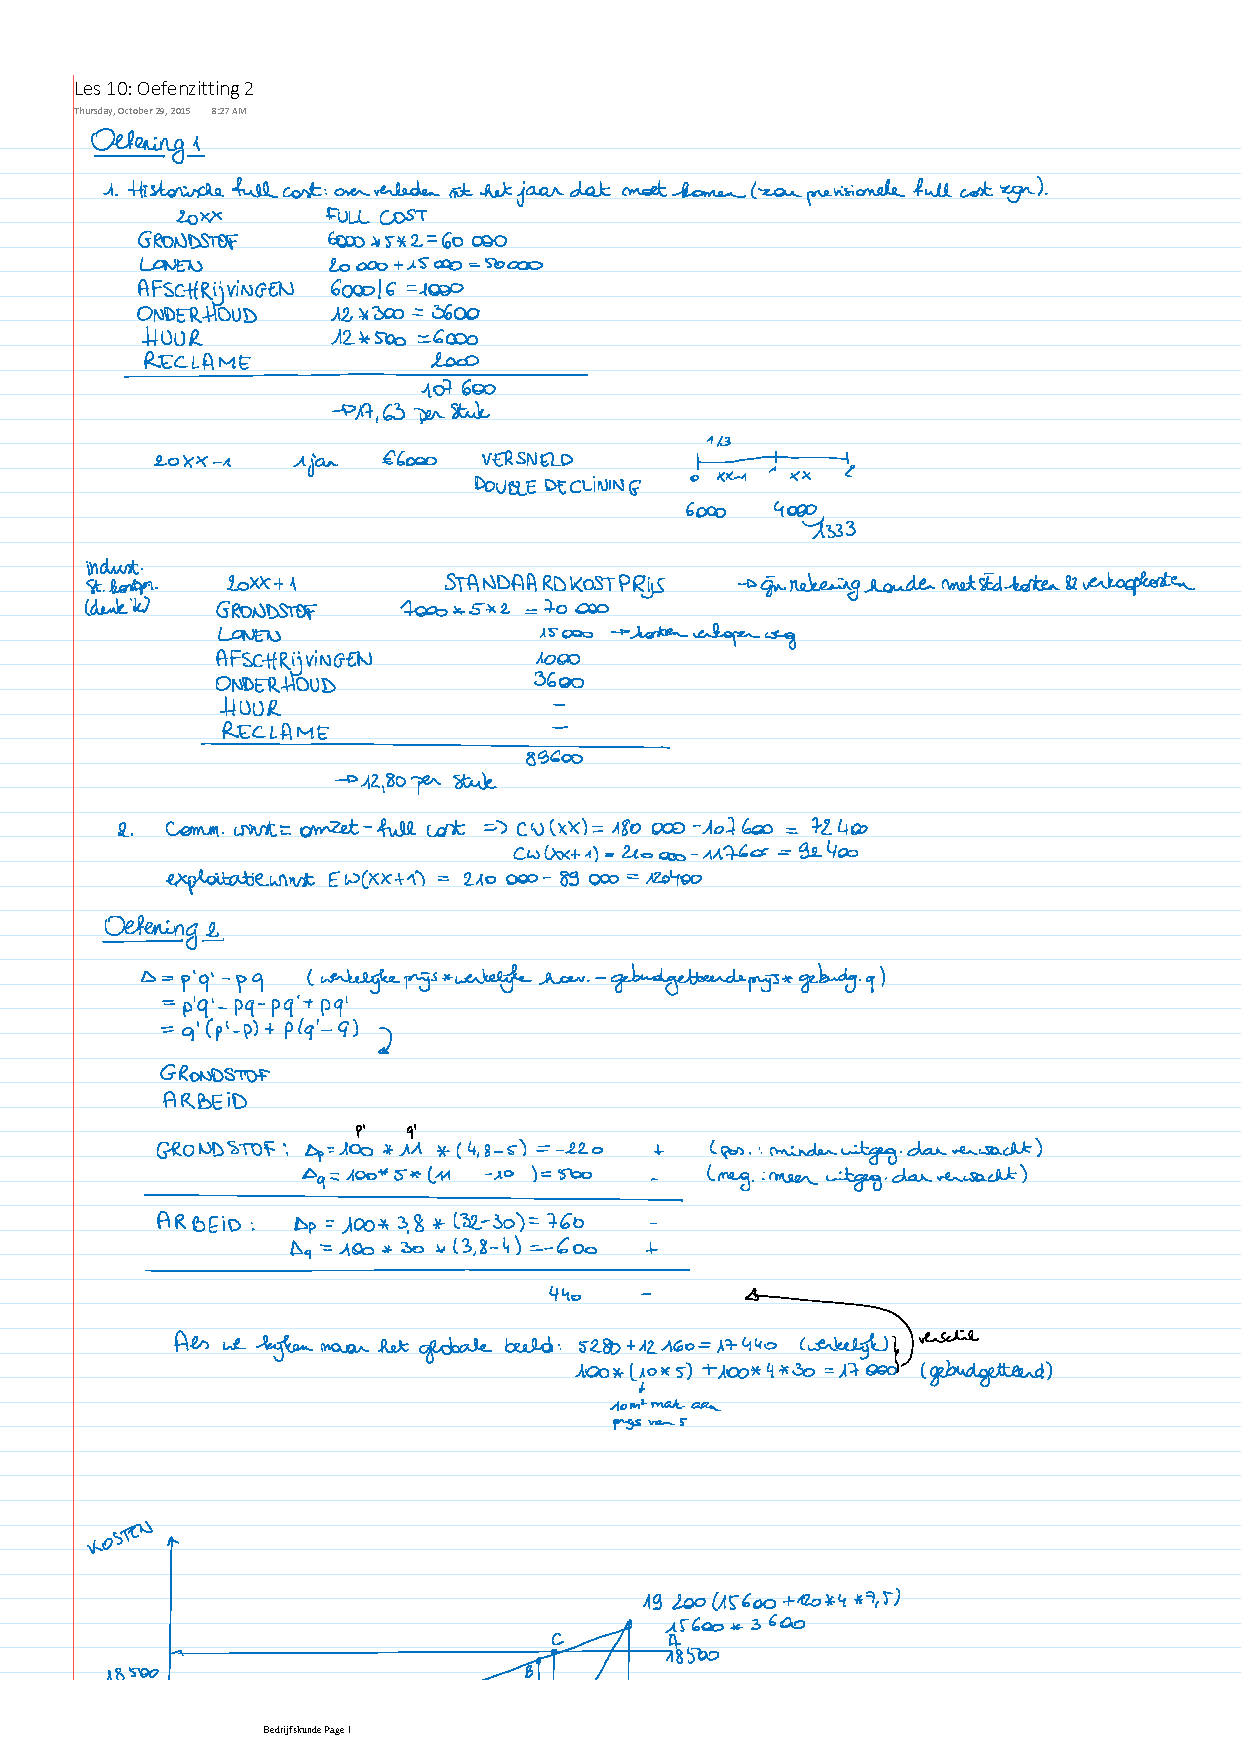
\includepdf[pages={1,2,3}]{Les10Oefenzitting2.pdf} 

\chapter{Les 11}

\section{Slides: 10\_Bedrijfskunde\_Voorspellingstechnieken}

\paragraph{Slide 25:} We gaan eerst kijken naar causale modellen: er gebeurt nu iets dat impact zal hebben op iets wat een paar maanden later gebeurt. We willen een verband leggen tussen wat nu gebeurt en wat later gebeurt.
Als er geen causaal verband is, maken we gebruik van tijdsreeksen gebaseerd op historische gegevens.\\
Belangrijk is om altijd een tekening te hebben als je historische gegevens hebt, zo kan je beter zien of er een trend is. De methode die je gebruikt zal afhankelijk zijn van het patroon dat je vindt. Als je een methode gebruikt die een trend niet kan weergeven, ga je een probleem hebben. Het is beter een methode te gebruiken die meer doet dan je verwacht. 

\paragraph{Slide 26:} D is de vraag in een bepaalde peroide, F is de voorspelling gemaakt op basis van de periodes op voorhand. Werken we met tijdsreeksen, baseren we ons op voorgaande vragen, rekening houdend met een bepaald gewicht. Naarmate de vraag verder in het verleden zit, zal het gewicht lichter zijn.

\paragraph{Slide 27:} We hebben een loodgieter die moet voorspellen hoeveel spanklemmen hij nodig gaat hebben. De eerste parameter is de onafhankelijke, de tweede is afhankelijk.

\paragraph{Slide 28:} De eerste methode die je kan gebruiken is lineaire regressie: de vraag die we hebben naar spanklemmen is een functie van het aantal bouwtoelatingen dat gegeven werd (h) vermenigvuldigd met een parameter b. We willen het volgende weergeven: zie Figuur \ref{les11_01}.\\

\begin{figure}[h!]
\centering
\includegraphics[width=90mm]{Les11_01.png}
\caption{Les 11 Slide 28} 
\label{les11_01}
\end{figure}

Let op dat je de juiste verbanden legt! Als kinderen meer tv kijken en ouders kopen meer paraplu's, is het een niet per s\'e het gevolg van het ander. Het kunnen alletwee gevolgen zijn van het feit dat het regent.

\paragraph{Slide 30:} Stellen we de gegevens van \textbf{Slide 29} grafisch voor, zien we inderdaad een lineair verband.\\
De bedoeling is nu om het snijpunt te vinden en dan de helling van de curve te vinden.\\
Hoe kunnen we dit doen? We kunnen dit op het zicht doen. Als we er een lijn doortrekken, kunnen we zien dat we starten op ongeveer 25. we hebben een stijging van ongeveer 300, dus ongeveer 1,85. Als je 100 bouwplannen krijgt, zal je 25+185=210 spanklemmen nodig hebben.

\paragraph{Slide 31:} We kunnen ook telkens de fout ten opzichte van de rechte berekenen.

\paragraph{Slide 32:} De formules om de fout te vinden. Het resultaat blijkt 1,83 te zijn, hoewel de schatting 1,85 was. Dit toont dat de grafische methode vaak al genoeg is. Op het examen moet je de formules dus ook niet per s\'e gebruiken, de grafische methode is soms voldoende.\\
Ex-examenvraag: je hebt als vraag 98, 100, 102, 104, 106, 108, wat is het volgende getal in de rij? Ga niet die formules gebruiken, je ziet dat het met 2 stijgt, dus het volgende getal is 110.

\paragraph{Slide 33:} Er zijn ook andere regressiemethoden.

\paragraph{Slide 34:} Causale modellen zijn interessant wanneer er een verband is waarbij je 1 onderdeel kent en het andere wilt voorspellen.\\
Let op dat de zaken die je gebruikt vaak enkel bruikbaar zijn binnen bepaalde marges. Als je voor een bepaalde grootte van het product maar 1 persoon nodig hebt aan de machine, kan het zijn dat als het product groter wordt, je 2 mensen nodig hebt, dus gaat uw curve niet meer kloppen.

\paragraph{Slide 35:} Dikwijls hebben we geen causaal model en moeten we ons baseren op basis van tijdsreeksen. We beginnen met stationaire tijdsreeksen: constante processen. We nemen aan dat de vraag constant is en epsilon gelijk is aan de ruis.

\paragraph{Slide 36:} We gaan kijken naar de vorige periodes, die vragen optellen en dan delen door het aantal. Je moet wel bepalen welke input je neemt en we gaan ook kijken naar de invloed van die N.

\paragraph{Slide 37:} We kijken naar de verkoop van tandpasta. 

\paragraph{Slide 38:} De vraag van tandpasta weergegeven. Als we de voorspelling zouden willen maken voor periode 51 op basis van 3 periodes: zie Figuur \ref{les11_02}.

\begin{figure}[h!]
\centering
\includegraphics[width=90mm]{Les11_02.png}
\caption{Les 11 Slide 38} 
\label{les11_02}
\end{figure}

\paragraph{Slide 40:} De donkere curve is het vraagpatroon. We hebben nog een gele en roze curve. Het driewekelijkse gemiddelde zal starten na 3 weken (dus roze), het zeswekelijkse gemiddelde zal na 6 weken starten. Het gele is daarenboven meer uitgevlakt en genereert een stabieler patroon dan het roze. In de gele curve neem je meer getallen mee, waardoor het meer uitgevlakt zal zijn. Als je 3 keer 10 neemt, krijg je een gemiddelde van 10. als je 10, 10, 20 neemt, krijg je 13,3. Als we zouden kijken naar 6 perioden, zal een afwijking (van die 10) veel minder uitgesproken zijn. 

\paragraph{Slide 41:} Kijken we naar dezelfde vraag waarbij de concurrentie in rekening genomen moet worden: we zien een stijging in de vraag. Kijken we hier naar de 2 patronen: het driewekelijks gemiddelde zal sneller reageren dan het zeswekelijks gemiddelde omdat in het driewekelijks gemiddelde getallen sneller `verdwijnen' (je neemt ze sneller niet meer in rekening), het zeswekelijks gemiddelde zal langer blijven werken met oudere getallen. Als er wijziigngen zijn, zal het zeswekelijks gemiddelde dus achterlopen op het driewekelijkse gemiddelde.

\paragraph{Slide 42:} Wanneer we trends hebben, zal het voortschuivend gemiddelde continu achterlopen bij een stijging en voorlopen bij een daling.

\paragraph{Slide 43:} Voordeel: stabiel. Nadelen: je moet kijken of er een trend is of niet en bepaalde zaken worden niet in rekening gehouden, zoals complexe relaties, die hierin niet kunnen worden meegenomen.

\paragraph{Slide 44:} Tweede techniek om stationaire reeksen te voorspellen: exponenti\"ele afvlakking. We gaan elke keer een gewogen gemiddelde berekenen: we maken een bepaalde voorspelling, krijgen een bepaalde vraag die normaal zal afwijken en we gaan dat lineair interpoleren en op basis daarvan een nieuwe vraag afleiden. Het komt er dus op neer dat we een gewogen gemiddelde nemen tussen de gekende vraag en de voorspelling. We moeten weer een gewicht geven aan de gekende vraag en het voorspelde getal. De nieuwe voorspelling zal gelijk zijn aan $\alpha$. 

\paragraph{Slide 45:} $\alpha$ zal men meestal leggen rond 0,1, 0,2. Als je $\alpha$ groter maakt, zal je veel meer variabel rondspringen. Als $\alpha$ kleiner is, zal je een veel stabieler patroon hebben. Als je de eerste formule uitschrijft als $F_{t-1}$ en $D_{t-1}$, zie je dat we rekening houden met alle voorbije data. De factor waarmee we rekening houden met het verleden wordt wel kleiner met de tijd. 

\paragraph{Slide 46:} Je ziet dat oude data steeds minder gewicht krijgt.
Voorbeeld: zie Figuur \ref{les11_03}.

\begin{figure}[h!]
\centering
\includegraphics[width=90mm]{Les11_03.png}
\caption{Les 11 Slide 46} 
\label{les11_03}
\end{figure}

\paragraph{Slide 47:} Als er een trend is, lopen beide methoden achter. ES houdt rekening met alle voorbije data, met telkens minder gewicht. Het grote voordeel van het voortschrijdend gemiddelde is dat als er ergens een piek is (meetfout bv.), dan zal die na enkele periodes niet meer in rekening genomen worden. 

\paragraph{Slide 48:} We hebben voor de voorbije 24 maanden de verkopen staan. Als we kijken naar de cijfers die er staan, merken we dat de waarden stijgen en er zal wellicht ergens een trend inzitten. We kunnen dit oplossen met regressieanalyse, maar expoleren is gevaarlijk.

\paragraph{Slide 49:} Komen we een curve zoals deze tegen, gaan we dubbele exponenti\"ele afvlakking gebruiken. Het is de bedoeling om de trend te vinden (lineair) die er is.

\paragraph{Slide 51:} Het komt erop neer dat wanneer we kijken naar een voorspelling, we ergens een startpunt hebben en ergens een bepaalde trend (zie tekening). Op basis van het startpunt en de trend zullen we uiteindelijk onze voorspelling bekomen. Zie Figuur \ref{les11_04}.\\

\begin{figure}[h!]
\centering
\includegraphics[width=30mm]{Les11_04.png}
\caption{Les 11 Slide 51 (1)} 
\label{les11_04}
\end{figure}

In de eerste vergelijking, $S_{t-1} + G_{t-1}$ komt overeen met $F_{t}$. Ons nieuw startpunt zal overeenkomen met de voorspelling aan de ene kant en de vraag aan de andere kant.\\
De volgende helling wordt bepaald door de trend van de vorige periode, het verschil tussen de twee startpunten (stippellijn op Figuur \ref{les11_05}). We zullen een weging maken tussen de oorspronkelijke trend en de trend veroorzaakt door de 2 startpunten. Dan vertrekken we daaruit en krijgen we $G_{t}$. Zie Figuur \ref{les11_05}.

\begin{figure}[h!]
\centering
\includegraphics[width=90mm]{Les11_05.png}
\caption{Les 11 Slide 51 (2)} 
\label{les11_05}
\end{figure}

\paragraph{Slide 52:} We willen een voorspelling maken. We moeten ergens op een of andere manier een startpunt vinden (S24) en een G24 zodanig dat al we S24 en G24 optellen, we F25 krijgen.\\
We kunnen dit op verschillende manieren doen: grafisch (lijn trekken en dan aflezen op de grafiek). We moeten hierbij dan een goede trend vinden en een start bepalen.\\
We hebben 2 jaren gegeven. De trend over 2 jaar heen is ongeveer dezelfde. Als we daarmee starten, kunnen we het volgende doen: zie Figuur \ref{les11_06}.\\

\begin{figure}[h!]
\centering
\includegraphics[width=90mm]{Les11_06.png}
\caption{Les 11 Slide 52 (1)} 
\label{les11_06}
\end{figure}

Kijken we naar deze cijfers: als je een overschatting maakt, gaat alles naar beneden getrokken worden, maak je een onderschatting, wordt alles naar boven getrokken. Zie Figuur \ref{les11_07}.\\

\begin{figure}[h!]
\centering
\includegraphics[width=90mm]{Les11_07.png}
\caption{Les 11 Slide 52 (2)} 
\label{les11_07}
\end{figure}

We kunnen dus op verschillende manieren starten. Wat we ook kunnen doen is Holt toepassen van in het begin. Je moet wel ergens een beginwaarde en begintrend vinden. Je kan dan een formule toepassen waarbij je de trend en het startpunt aanpast en zo een nieuw punt vindt. De voorspelling is dus de som van uw trend en uw startpunt.\\
Nu is het zo dat je andere waarden kan nemen als beginwaarde, dan zal je merken dat op het einde de afwijking relatief klein is. Als je in het begin ergens een fout hebt gemaakt, zal zich dat uitvlakken omdat oude informatie steeds minder hard zal doorwegen. 

\paragraph{Slide 53:} We hebben ook seizoensinvloeden. Het is dan interessant om te kijken naar de periodes waarin ze terugkeren. Je kan seizoensinvloeden hebben die over een jaar zijn (bv. Speelgoedfabrikanten), maar ook om de zoveel maanden. Je moet dit eerst proberen te herkennen vanuit uw data. Dan ga je een formule opstellen.

\paragraph{Slide 55:} We gebruiken altijd hetzelfde systeem: we hebben ergens een bepaald startpunt, een bepaalde trend en dan krijg je een punt op de trendlijn en moet je de seizoensfactor introduceren (factor $>$1 of $<$1). In dit geval hebben we een seizoensinvloed die gekoppeld is aan een trend. Zie Figuur \ref{les11_08}.

\begin{figure}[h!]
\centering
\includegraphics[width=90mm]{Les11_08.png}
\caption{Les 11 Slide 55} 
\label{les11_08}
\end{figure}

\paragraph{Slide 56:} Gelijkaardige formules. $S_{t}$ = startpunt, $G_{t}$ = de helling, $c_{t}$ = seizoensinvloed. We gaan de vraag delen door de seizoensfactor (D/c) zodat we het verschil hebben.\\
Als het vraagpatroon er als volgt zou uitzien, dan gaan we niet de zwarte periodes nemen. We gaan het eerste deel aan de kant laten liggen, die zijn niet representatief. Het kan zijn dat je pas na een tijd een normale vraag krijgt. \\

\begin{figure}[h!]
\centering
\includegraphics[width=90mm]{Les11_09.png}
\caption{Les 11 Slide 56} 
\label{les11_09}
\end{figure}

Als je het eerste deel meeneemt, ga je te lang nodig hebben om je aan te passen en de fout weg te werken.

\paragraph{Slide 58:} Formules.

\paragraph{Slide 59:} Voorbeeld: We hebben de periodes t, de vraag d en de voorspelling F gekoppeld aan die vraag d. e = F-d. E is de cumulatieve fout. MAD is de absolute waarde van het gewogen gemiddelde. MSE is de gemiddelde foutmarge in het kwadraat. MAPE zijn de percentages.\\
Wat kunnen we zeggen over de e-kolom? We moeten zowel positieve als negatieve waarden hebben. Als we altijd een positieve of negatieve fout vinden, gaan we voorlopen. Het is niet zo dat we graag kleine negatieve en grote positieve waarden hebben. We willen dat als we de som gaan bekijken, we ongeveer 0 uitkomen. Als de waarden in E zowel positief als negatief zijn, is dat ook goed. Je wilt waarden vinden die positief en negatief zijn en liefst zo dicht mogelijk bij nul liggen. Bij MAD, MSE en MAPE hebben we graag waarden die stabiel worden na een bepaalde periode. Kijken we naar de gemiddelde fout en de gemiddelde kwadratische fout, deze mogen niet plots beginnen stijgen, want dan krijgen we plots grote afwijkingen. We willen dus dat die waarden relatief stabiel zijn. MAPE moet ook stabiel zijn, dat geeft ons weer wat onze gemiddelde afwijking is.\\
Als we tot de conclusie komen dat bepaalde zaken totaal fout lopen, moeten we de zaken analyseren.

\paragraph{Slide 60:} Bias: constant positief of negatief. 

\paragraph{Slide 61:} Om dit te kunnen opvolgen maakt men gebruik van quality management. We willen dat onze fout binnen een bepaalde marge zit (komt niet op examen, ter informatie). Er is een verband tussen de gemiddelde absolute afwijking en de $\sigma$ van de ruis. De $\sigma$ van de ruis is ongeveer de gemiddelde afwijking/0,8. Voor de $\alpha$-waarden kom je dan ook tot een bepaald verband.\\
Uiteindelijk is het zo dat we ergens een fout zullen maken en dat we proberen die fout te krijgen tussen 2 waarden. Zolang onze fout tussen die twee waarden zit, zullen we aannemen dat onze voorspellingstechniek goed werkt. Zitten we buiten die waarden, dan moeten we gaan reageren en nakijken wat er verkeerd loopt met onze methode of wat er is aangepast aan het vraagpatroon. 

\paragraph{Slide 62:} Om dit te kunnen doen, maken we voorspellingen op de fouten. Zolang $\rho$ kleiner of gelijk is aan 4, zitten we goed. 

\paragraph{Slide 64:} We gaan de voorspellingen genereren en doorrekenen. We zien dan dat $\rho$ altijd kleiner is dan 4. In dit geval zitten we betrouwbaar en hebben we geen enkel probleem. Onze voorspellingsmethode werkt dus goed.

\paragraph{Slide 66:} Bij exponenti\"ele afvlakking zijn er problemen als er een plotse sprong is. Exponenti\"ele afvlakking kan het dus niet volgen.\\
We doen dezelfde berekeningen (\textbf{Slide 67}) en zien dat onze delta (voorspelling van de fout) dit toont, alsook rho: rho komt boven de 4. Als je dat merkt, wil dat zeggen dat je moet reageren, je moet nakijken wat er fout loopt.\\
Wil het zeggen dat als je boven 4 zit, er een foute methode wordt gebruikt? Niet noodzakelijk. Het kan zijn dat er iets gebeurd is waardoor we plots een grote rho krijgen. Het kan zijn dat er een sprong is geweest, maar achteraf opnieuw een stabiel patroon. We moeten gewoon kijken wat er gebeurd is, en eventueel geen rekening houden met die sprongen. 

\paragraph{Slide 68:} Je moet niet plots nieuwe methoden gebruiken, gewoon eerst kijken wat er gebeurd is en dan handelen. Je kan dan bepaalde cijfers schrappen en initaliseren met nieuwe waarden.\\
Kijken we op het einde naar de waarden (\textbf{Slide 67}), zien we rho weer dalen naar het einde toe.

\paragraph{Slide 70:} Het is van groot belang om na te gaan welk model gebruik moet worden. Je moet dit ook opvolgen, niet gewoon starten en dan zo verder werken, je moet altijd controleren.\\
We hebben zeer eenvoudige modellen gezien, er zijn er natuurlijk ook complexere. 

\paragraph{Slide 72:} Onze voorspelling zal juist zo zijn dat we die nodig hebben voor onze voorraadbeheer en ons productieplan. Kijken we naar de voorraad, kijken we naar de eindvoorraad. Als die eindvoorraad is vastgelegd, gaan we daaraan de productie koppelen. Bij de inventory gaan we andere assumpties maken dan bij de productie.

\chapter{Les 12}
\section{Slides: 11\_Bedrijfskunde\_Productie- en voorraadcontrolesystemen(1)}

\paragraph{Slide 2:} We gaan een voorraadpolitiek vastleggen. Op basis daarvan kijken we naar het productieplan zelf. De eerste 4 systemen worden allemaal gebruikt om productie aan te sturen. 

\paragraph{Slide 4:} Voorraadbeheer is van belang omdat de verkoop (en voorraad) gekoppeld is aan de financi\"ele cyclus van het bedrijf. We willen dat de voorraadrotatie klein is zodat de financi\"ele cyclus ook klein is. Het is de bedoeling dat de cirkel zo snel mogelijk rond is en het geld zo snel mogelijk opnieuw binnenkomt.

\paragraph{Slide 5:} We gaan kijken naar voorraden omdat zelfs als de vraag volledig deterministisch en gekend zou zijn, we toch gebruik gaan maken van voorraden. De redenen zijn gegeven in het lijstje:
\begin{itemize}
\item Schaalvoordelen: naarmate we meer stuks maken, kunnen we de vaste kosten verdelen over al die stuks, waardoor de kost per stuk lager is: zie Figuur \ref{les12_01}.

\begin{figure}[h!]
\centering
\includegraphics[width=90mm]{Les12_01.png}
\caption{Les 12 Slide 5 (1)} 
\label{les12_01}
\end{figure}	
	
\item Onzekerheid in levertermijn: er zit een bepaalde spreiding op wanneer de leverancier levert. Je moet zorgen dat als de leverancier aan de late kant is, je toch nog kan produceren.
\item Speculatie: als je weet dat accijnzen bv. gaan stijgen, ga je voorraden aanleggen.
\item Transport
\item Uitvlakken productie: zie Figuur \ref{les12_02}.

\begin{figure}[h!]
\centering
\includegraphics[width=90mm]{Les12_02.png}
\caption{Les 12 Slide 5 (2)} 
\label{les12_02}
\end{figure}

\item Logistiek
\item Controlekosten: je moet betalen per controle, dus als je meer kan laten controleren in een keer, zal het goedkoper zijn.
\end{itemize}

\paragraph{Slide 6:} We moeten altijd controleren hoe we verkopen: soms meer, soms minder. We moeten continu controleren wat er gebeurt met de voorraad. 

\paragraph{Slide 7:} Er bestaan verschillende systemen. Het eerste gaat periodiek kijken wat er gebeurt met de voorraad. Ongeacht wat er gebeurt, we gaan pas kijken op $t_{1}$ en daarna op $t_{2}$. We merken dat we een target niveau hebben (max. niveau van voorraad dat we willen), maar ook een reorder point: zodra we hieronder komen, gaan we bijbestellen. De restvoorraad zal onvoldoende zijn om de cyclus te overbruggen. Je bemerkt dat we controleren op $t_{1}$ en $t_{2}$, bij $t_{2}$ zien we dat we moeten bijbestellen. Het kan ook zijn dat de voorraad veel drastischer gaat dalen, waarbij je negatieve voorraad kan hebben, waarbij je niet kan voldoen aan de vraag. \\
Een ander systeem is het continu herzien: continu kijken in ons magazijn hoe de voorraad is. We zien dat onze voorraad daalt en dat we ons reorder point naderen, dus we gaan opnieuw bijbestellen. Als de voorraad nu heel snel daalt, gaan we snel kunnen bijbestellen. \\
Het systeem van continu herzien zal veel duurder zijn dan periodiek herzien. Men gebruikt bij continu herzien vaak RFID of barcodes. Men zal continu herzien gebruiken voor kritieke stukken, wanneer tekorten daarbij grote implicaties heeft voor de klanten. Voor standaardstukken ga je periodiek herzien gebruiken, waarbij het wel eens (een beetje) mag foutlopen.

\paragraph{Slide 8:} Aan de ene kant is het nuttig om zoiets te hebben omdat we zo flexibel kunnen zijn, maar anderzijds gaan we ook een hele reeks kosten hebben. Die kosten hebben te maken met
\begin{itemize}
\item opslag: daar zit geld in dat niet gebruikt kan worden. Dit wordt dikwijls uitgedrukt in procenten: hoeveel procent van de voorraad zal voor een bepaalde bestelling gebruik worden?
\begin{itemize}
\item Verouderingskosten: als producten ergens lang liggen, gaan klanten dat misschien niet meer willen. Het kan zijn dat er producten zijn die niet meer roteren in het bedrijf. Ze zijn niks meer waard voor de klant, maar het bedrijf houdt ze omdat ze anders de balans moeten aanpassen.
\item Diefstal: als er taarten worden gemaakt in de winkel, kan het zijn dat het personeel versieringen ofzo zelf opeet.
\end{itemize}
\item voorraadbreukkosten: het kan zijn dat men zegt dat er per dag te laat een bepaalde boete betaald wordt, of dat je die klant verliest. Op die manier kan je eventueel ook andere klanten verliezen omdat je niet betrouwbaar bent. Je kan werken met een service graad: men gaat proberen een voorraadniveau te halen zodat je in 95\% van de gevallen kan leveren aan je klant.
\item orderkosten: gegevens ingeven, kijken wat er gebeurt aan de los- en laadkade.
\item Opvolging: software/hardware om bv. te kijken welke boeken in een bibliotheek binnenkomen/buitengaan kost ook geld.
\end{itemize}

\paragraph{Slide 9:} Als we kijken naar kosten moeten we 2 zaken afwegen: voorraadkosten en naarmate de lotgrootte stijgt, zullen we grotere voorraden krijgen. Kleinere batches zorgen voor kleinere voorraadkosten, maar dit kan zorgen voor grotere omstelkosten (== bestelkosten). Het is de bedoeling om die 2 tegenover elkaar af te wegen. Als je de totale kost neemt, ga je het minimum zoeken en dat is het punt waarbij je totaal genomen de kleinste voorraadkost en bestelkost hebt. 

\paragraph{Slide 10:} We hebben verschillende soorten modellen. Wij gaan enkel kijken naar de statische modellen. Voor de dynamische heb je modelleringsmodellen nodig.\\
We gaan voorbeelden bekijken waarbij we kijken naar uniforme constante vraag over de tijdshorizon. Hierbij gaan we kijken naar het eindprodcut en niet naar de onderliggende delen. %TODO Als jenaar de onderliggende delen kijkt (? 17.00).

\paragraph{Slide 11:} We beginnen met het basismodel. We nemen aan dat de vraag gekend, deterministisch en constant is. De lotgrootte q gaan we proberen te betalen. Deze is constant en wordt bijgesteld wanneer nodig. De voorraad wordt bijgevuld wanneer het voorraadniveau 0 is. We nemen aan dat de doorlooptijd om de voorraad heraan te leggen 0 is (dus nieuwe voorraad wordt besteld en is direct in huis).

\paragraph{Slide 12:} Zaagtandpatroon: elke keer als de voorraad 0 is, bestellen we bij. Dan halen we producten uit het magazijn. De vraag is cst dus het verloopt lineair. We gaan een bepaalde cyclus hebben en na periode T bestellen we bij. \\
We hebben voorraadkosten die gekoppeld zijn aan de batchkosten en de periodes T. Die gaan we moeten afwegen tegenover elkaar.\\ 
Kijken we naar onze gegevens, dan hebben we een bepaalde kost r, we kopen het product aan aan een kost c. We merken dat die totaal onafhankelijk is van onze batchgrootte (we krijgen geen korting bij grotere hoeveelheden). Dat is onze aankoopkost. We zullen een orderkost hebben en een voorraadkost. De voorraadkost is gegeven en de orderkost ook (op de vorige slide). De vraag is nu wat de voorraadkost is. Zie Figuur \ref{les12_03}.\\

\begin{figure}[h!]
\centering
\includegraphics[width=90mm]{Les12_03.png}
\caption{Les 12 Slide 12 (1)} 
\label{les12_03}
\end{figure}

We willen de jusite waarden vinden voor A, dus: zie Figuur \ref{les12_04}.\\

\begin{figure}[h!]
\centering
\includegraphics[width=90mm]{Les12_04.png}
\caption{Les 12 Slide 12 (2)} 
\label{les12_04}
\end{figure}

Naarmate de orderkost groter wordt, willen we minder bestellingen plaatsen, dus grotere batches (vandaar $c_{p}$ in de teller). Als de voorraadkosten groter worden, gaan we minder voorraad willen hebben, dus daarom $c_{h}$ in de noemer.\\
Bekijken we een paar specifieke zaken verder: zie Figuur \ref{les12_05}.

\begin{figure}[h!]
\centering
\includegraphics[width=90mm]{Les12_05.png}
\caption{Les 12 Slide 12 (3)} 
\label{les12_05}
\end{figure}

\paragraph{Slide 14:} De vraag is gekend, dus je kijkt hoe lang het duurt voor je voorraad voor x dagen opgebruikt is. Je bestelt op voorhand zodat je geen voorraadtekort krijgt.

\paragraph{Slide 15:} Je moet ervoor zorgen dat alle gegevens er staan met de juiste dimensies. Spreken we over jaarvragen, moeten we ook kijken naar jaarlijkse opportuniteitskosten. We gaan het voorbeeld uitwerken:

\begin{figure}[h!]
\centering
\includegraphics[width=90mm]{Les12_06.png}
\caption{Les 12 Slide 15 (1)} 
\label{les12_06}
\end{figure}

\begin{figure}[h!]
\centering
\includegraphics[width=90mm]{Les12_07.png}
\caption{Les 12 Slide 15 (2)} 
\label{les12_07}
\end{figure}

\paragraph{Slide 16 e.v.:} Marvin kan beter meer bestellen.

\paragraph{Slide 18:} We kunnen ook zelf onderdelen gaan produceren, maar dan zijn die onderdelen niet meteen beschikbaar, het duurt een bepaalde tijd vooraleer ze geproduceerd zijn. De vraag is nu of onze productiebatch groter of kleiner gaat zijn. Nemen we in de piek H als de hoogte van de voorraad: zie Figuur \ref{les12_08}. \\

\begin{figure}[h!]
\centering
\includegraphics[width=90mm]{Les12_08.png}
\caption{Les 12 Slide 18 (1)} 
\label{les12_08}
\end{figure}

Als p oneindig is, zijn die twee aan elkaar gelijk (q en H).
We kunnen de formule dus omvormen tot: zie Figuur \ref{les12_09}.\\

\begin{figure}[h!]
\centering
\includegraphics[width=90mm]{Les12_09.png}
\caption{Les 12 Slide 18 (2)} 
\label{les12_09}
\end{figure}

p moet groter zijn dan r, anders kan de productie niet voldoen aan de vraag.

\paragraph{Slide 20:} We kijken eerst naar een systeem waarbij we korting krijgen voor alle eenheden die we aankopen, daarna naar modellen waarbij we korting krijgen vanaf een bepaalde hoeveelheid.\\
Kijken we naar een verduidelijkend voorbeeld: zie Figuur \ref{les12_10}.

\begin{figure}[h!]
\centering
\includegraphics[width=90mm]{Les12_10.png}
\caption{Les 12 Slide 20 (1)} 
\label{les12_10}
\end{figure}

De $r_{c}$ zal nu wel vari\"eren, zal een functie zijn van q. hier zal het dus afhankelijk zijn van onze bestelgrootte.\\
Als we aannemen dat de drie kostenfuncties alledrie geldig zijn en we tekenen de volledige kostenfunctie uit, dan merken we dat we 3 curvers hebben, waarbij die met de hoogste aankoopkost bovenaan ligt en de laagste aankoopkost onderaan. Die curvers snijden elkaar niet in de tweede figuur. De curves zijn enkel geldig in de gemarkeerde gebieden: zie Figuur \ref{les12_11}.\\

\begin{figure}[h!]
\centering
\includegraphics[width=90mm]{Les12_11.png}
\caption{Les 12 Slide 20 (2)} 
\label{les12_11}
\end{figure}

Hoe kunnen we nu starten om de optimale oplossing te vinden? \\
De drie curves snijden mekaar niet en $c_{3}$ is de laagste en de andere twee liggen erboven. Als dit voldoet aan de voorwaarden, moet je de andere curven niet meer bekijken want het optimum ligt in het minimum van $c_{3}$. We zullen dus onderaan starten met de derde curve en kijken of dat optimale punt voldoet aan de eisen. Als het aan de rand ligt zoals op de afbeelding, zijn we niet zeker of het laagste punt daar lager ligt dan bij de tweede laagste. Is dit buiten het bruikbaar gebied, ga je weer naaar boven werken.\\
We bemerken ook dat als we de 3 curves met elkaar vergelijken, dan verschuift het minimum naar links. \\
Als we de curven tekenen en de aankoopkosten wijzigen, dan wijzigen ook de curven. Als de aankoopkost daalt, daalt de voorraadkost, zal de optimale hoeveelheid stijgen: zie Figuur \ref{les12_12}.\\

\begin{figure}[h!]
\centering
\includegraphics[width=90mm]{Les12_12.png}
\caption{Les 12 Slide 20 (3)} 
\label{les12_12}
\end{figure}

Voorbeeld: zie Figuur \ref{les12_13}.\\

\begin{figure}[h!]
\centering
\includegraphics[width=90mm]{Les12_13.png}
\caption{Les 12 Slide 20 (4)} 
\label{les12_13}
\end{figure}

We hebben hier dus het minimum van de onderste curve genomen.\\
We zijn niet zeker dat we het optimale punt hebben, dus we berekenen $q_{2}^{*}$: zie Figuur \ref{les12_14}. \\

\begin{figure}[h!]
\centering
\includegraphics[width=90mm]{Les12_14.png}
\caption{Les 12 Slide 20 (5)} 
\label{les12_14}
\end{figure}

Bij $q_{*}^{3}$ kopen we voor meer dan een jaar aan voorraad, je moet dan zeker zijn dat er geen plotse daling in verkopen zal zijn. Soms is het dus beter om het duurdere ($q_{2}^{*}$ in dit geval) te nemen, omdat je minder voorraad zal overhebben. Een verschil van 5 is vrij klein, dus het is zeker werkbaar. Je moet altijd kijken naar alle factoren. In dit geval is het dus beter om iets meer te betalen maar minder lang met voorraden te zitten.

\paragraph{Slide 21:} Bij incrementele korting gaan de curves mekaar snijden. Men heeft kunnen bewijzen dat de snijpunten nooit optimaal kunnen zijn. We gaan intu\"itief bekijken hoe de formule in elkaar zit.
We moeten alle kostencurves doorrekenen en enkel de kostencurves waarbij we een optimum vinden binnen de marges, daarmee gaan we verder werken. We gaan hier ook werken met de EOQ-formule.\\
Uw voorraadwaarde gaat hier niet meer lineair zijn zoals bij alle eenheden die korting krijgen.\\
We komen tot volgende formule: zie Figuur \ref{les12_15} $\&$ \ref{les12_16}.

\begin{figure}[h!]
\centering
\includegraphics[width=90mm]{Les12_15.png}
\caption{Les 12 Slide 21 (1)} 
\label{les12_15}
\end{figure}

\begin{figure}[h!]
\centering
\includegraphics[width=90mm]{Les12_16.png}
\caption{Les 12 Slide 21 (2)} 
\label{les12_16}
\end{figure}

\paragraph{Slide 22:} Dikwijls zal het zo zijn dat er beperkingen zijn (we hebben niet maar 1 product bv.) en zal er interactie zijn tussen verschillende systemen. We gaan hierbij gebruik maken van lagrange-relaxatie. Zie Figuur \ref{les12_17}.

\begin{figure}[h!]
\centering
\includegraphics[width=90mm]{Les12_17.png}
\caption{Les 12 Slide 22} 
\label{les12_17}
\end{figure}

Je kan lambda bepalen, maar de noemers zijn aan elkaar gelijk. Wanneer je zit met een budgetbeperking, zal die evenredig zijn over de verschillende producten (denk ik).\\
We vinden dat $q_{1}$ = 36 en $q_{2}$ = 40. Ze zijn op een gelijkaardige manier gedaald. \\
Op die manier kan men relaties inbrengen waarbij producten aan elkaar gekoppeld zijn. Men kan ook meerdere beperkingen inbouwen.


\end{document}